\documentclass{beamer}
\setbeamertemplate{navigation symbols}{}
%\usetheme{Goettingen}
\usetheme{Malmoe}
\usefonttheme{default}
%\setbeamersize{text margin left=5pt,text margin right=5pt}

\usepackage{hyperref}
\usepackage{subfigure}
\usepackage{amsmath}
\usepackage{amssymb}
\usepackage{multimedia}
\usepackage{shadow}
%\usepackage{movie15}

\usepackage{tcolorbox}

% Create a ``Wider'' command to reduce margins.  Put
% ``\Wider{\lipsum[2]}'' in a frame...
\newcommand\Wider[2][3em]{%
\makebox[\linewidth][c]{%
  \begin{minipage}{\dimexpr\textwidth+#1\relax}
  \raggedright#2
  \end{minipage}%
  }%
}

\tcbset{ % colback=blue!5,colframe=blue!75!black,
    noparskip,
    colback=blue!5, %background color of the box
    colframe=blue!70, %color of frame and title background
    coltext=black, %color of body text
    coltitle=black, %color of title text 
    fonttitle=\bfseries,
    update/.style={coltitle=red, 
                     colframe=gray!40},
    quote/.style={coltitle=gray!20, 
                     colframe=black,             
                     colback=green!5},
    }


%\usepackage[english]{babel}
%\usepackage{pgf,pgfarrows,pgfnodes,pgfautomata,pgfheaps}
% \usepackage[latin1]{inputenc}

\usepackage{graphicx}
\defbeamertemplate*{footline}{default theme}
{
  \leavevmode%
  \hbox{%
  \begin{beamercolorbox}[wd=.5\paperwidth,ht=2.25ex,dp=1ex,center]{author in head/foot}%
    %\usebeamerfont{author in head/foot}\insertshortauthor~~(\insertshortinstitute)
    \usebeamerfont{author in head/foot}\insertshortauthor
  \end{beamercolorbox}%
  \begin{beamercolorbox}[wd=.4\paperwidth,ht=2.25ex,dp=1ex,center]{title in head/foot}%
    \usebeamerfont{title in head/foot}\insertshorttitle
  \end{beamercolorbox}%
  \begin{beamercolorbox}[wd=.1\paperwidth,ht=2.25ex,dp=1ex,right]{date in head/foot}%
%    \usebeamerfont{page number}\insertframenumber{} / \inserttotalframenumber\hspace*{2ex} 
    \usebeamerfont{page number}\insertpagenumber{} / \insertpresentationendpage{} \hspace*{2ex} 
  \end{beamercolorbox}}%
  \vskip0pt%
}

\title[Transportation]{Transportation}

\author{Ben Pearre}
%\institute[]{
%  Computer Science\\
%  University of Colorado at Boulder, USA}
\date{\today}
%\date{\today}

\begin{document}

%\begin{frame}
%  \titlepage
%\end{frame}

%\begin{frame}
%  \frametitle{Outline}
%  \tableofcontents
%\end{frame}


\section{Macmillan {\it et al.} 2014}

\subsection{Authors}

\begin{frame}
  \frametitle{The Societal Costs and Benefits of Commuter Bicycling}
  \begin{columns}
    \column{0.5\textwidth}
    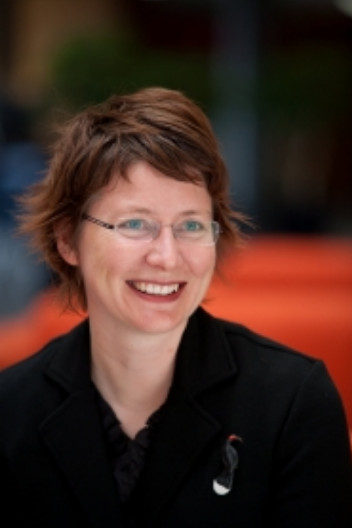
\includegraphics[height=0.3\textheight]{AlexMacmillan.jpg}
    \begin{itemize}
    \item Alexandra Macmillan
    \item University of Otego: Preventive and Social Medicine
    \item PhD: University of Auckland, 2012
    \end{itemize}
    \column{0.5\textwidth}
    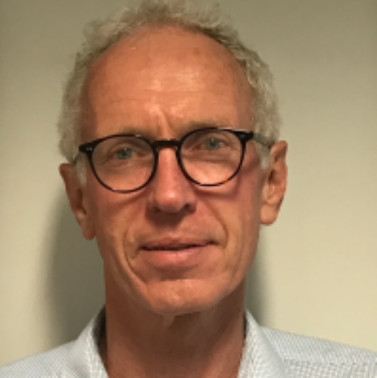
\includegraphics[height=0.3\textheight]{AlistairWoodward.jpg}
    \begin{itemize}
    \item Alistair Woodward
    \item University of Auckland: Medical and Health Sciences
      \begin{itemize}
      \item Head of School of Population Health 2004--2012
      \end{itemize}
    \end{itemize}
  \end{columns}
\end{frame}

\begin{frame}
  \frametitle{More authors!}
  \begin{description}
  \item[Jennie Connor] U of Otego, Dunedin, Department of Preventative and Social Medicine
  \item[Karen Witten] Massey U, Auckland, Social and Health Outcomes Research and Evaluation
  \item[Robin Kearns] U of Auckland, School of Environment
  \item[David Rees] Synergia Ltd, Auckland
  \end{description}
  \vskip 5 mm
  Environmental Health Perspectives: impact factor $\approx 8$
\end{frame}

\subsection{Why?}

\begin{frame}
  \frametitle{Why bike?}
  \begin{itemize}
  \item Health
  \item Social equity
  \item Minimise expenses
  \item Pollution / climate
  \end{itemize}
  \vskip 5 mm
  Objective:   Increase bicycling in a car-dominated city
\end{frame}

\subsection{Model}

\begin{frame}
  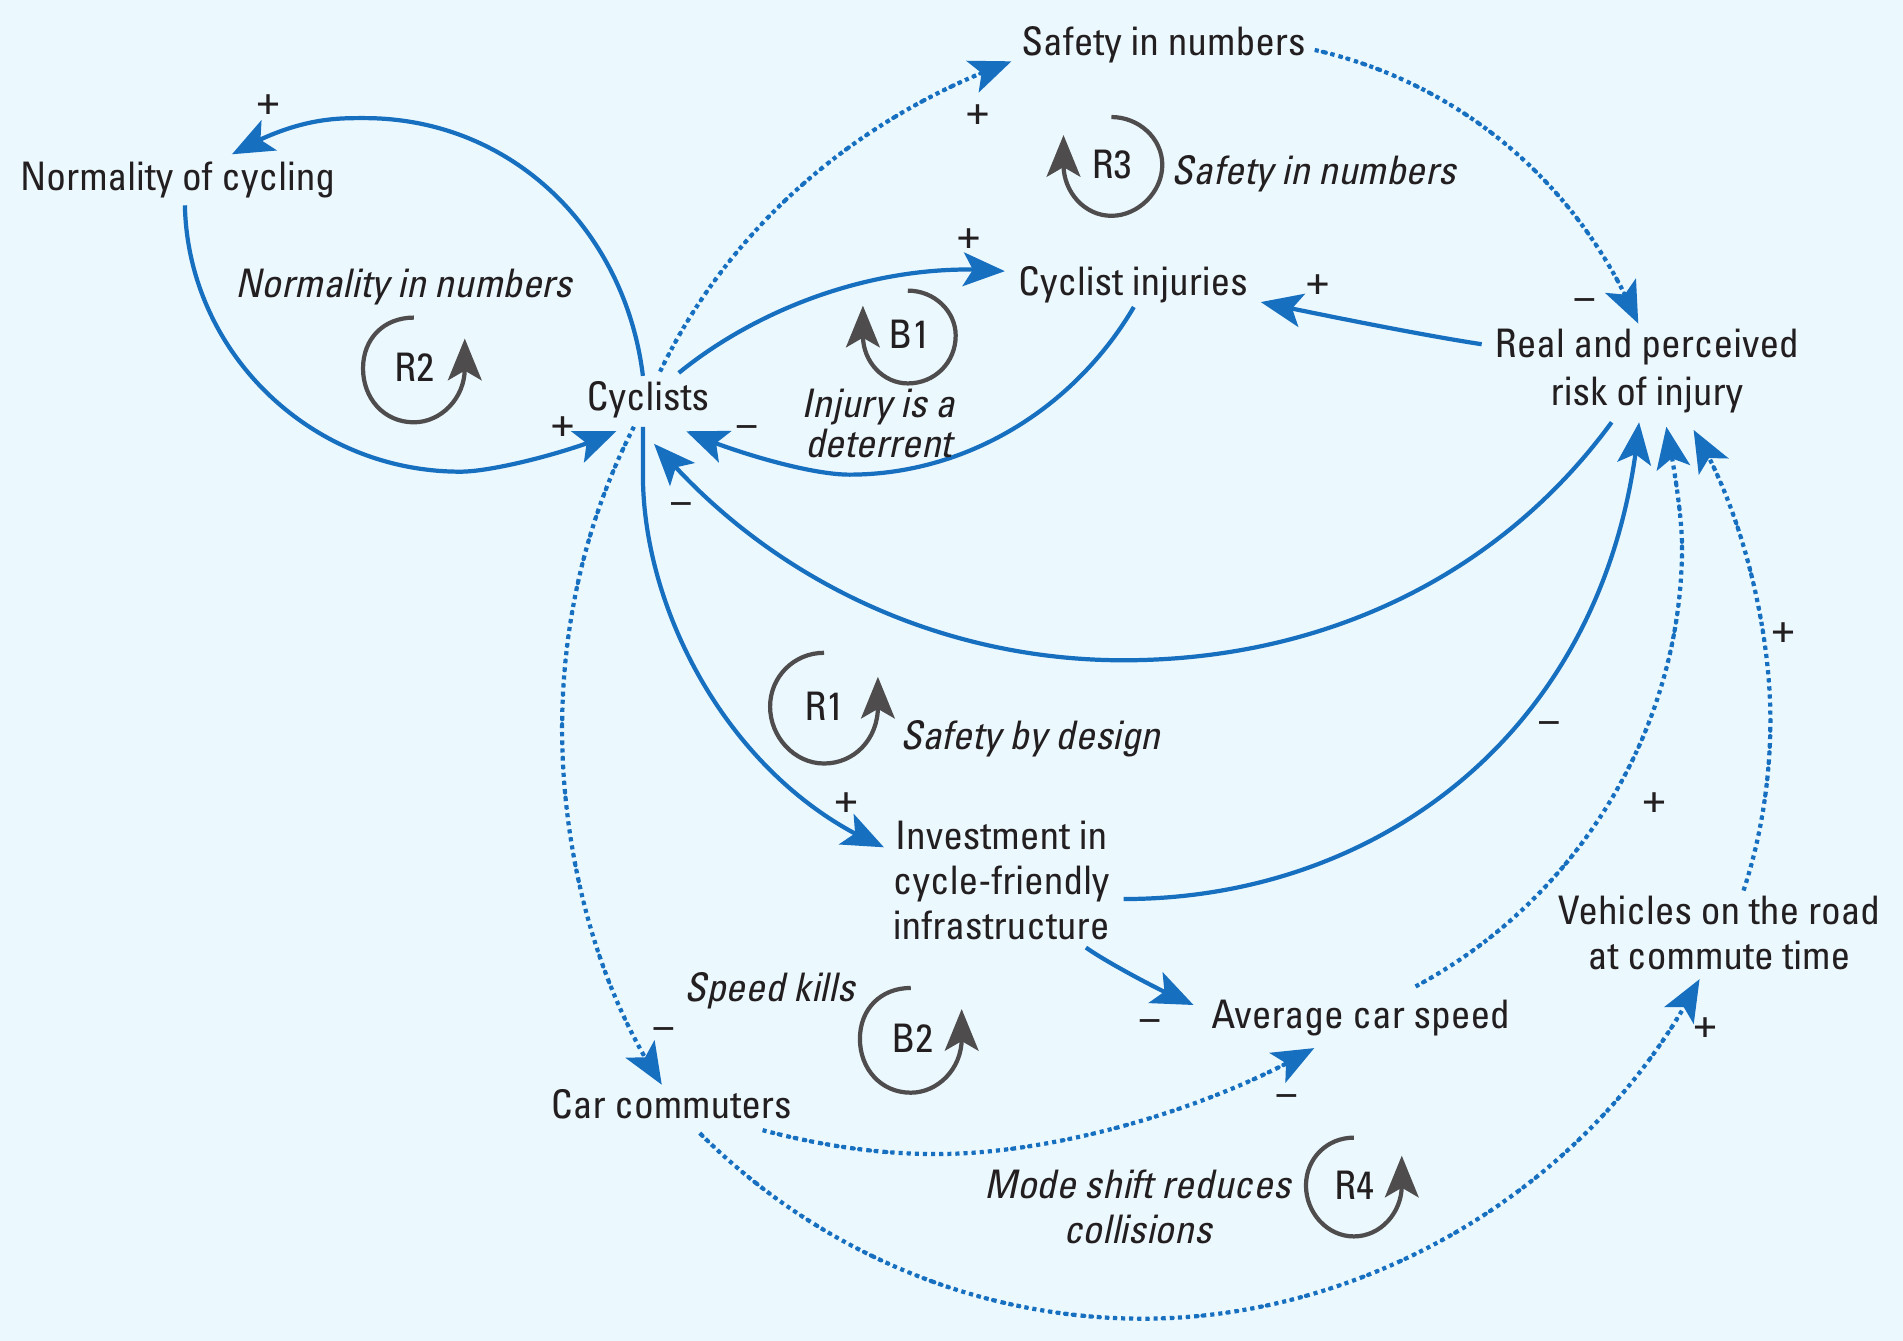
\includegraphics[width=\textwidth]{Macmillan-sd-model.jpg}
\end{frame}

\begin{frame}
  \frametitle{Details}
  \begin{itemize}
  \item Population 400,000, growing 40\%, same demographic
  \item Light vehicle 0.85, bicycling 0.02, walking 0.055, public transport 0.075
  \item Bikeable: $\le 6$ km (50\%). Walkable: $\le 2$ km (27\%).
  \item Bike commuting relative risk: 0.72
  \end{itemize}
\end{frame}

\begin{frame}
  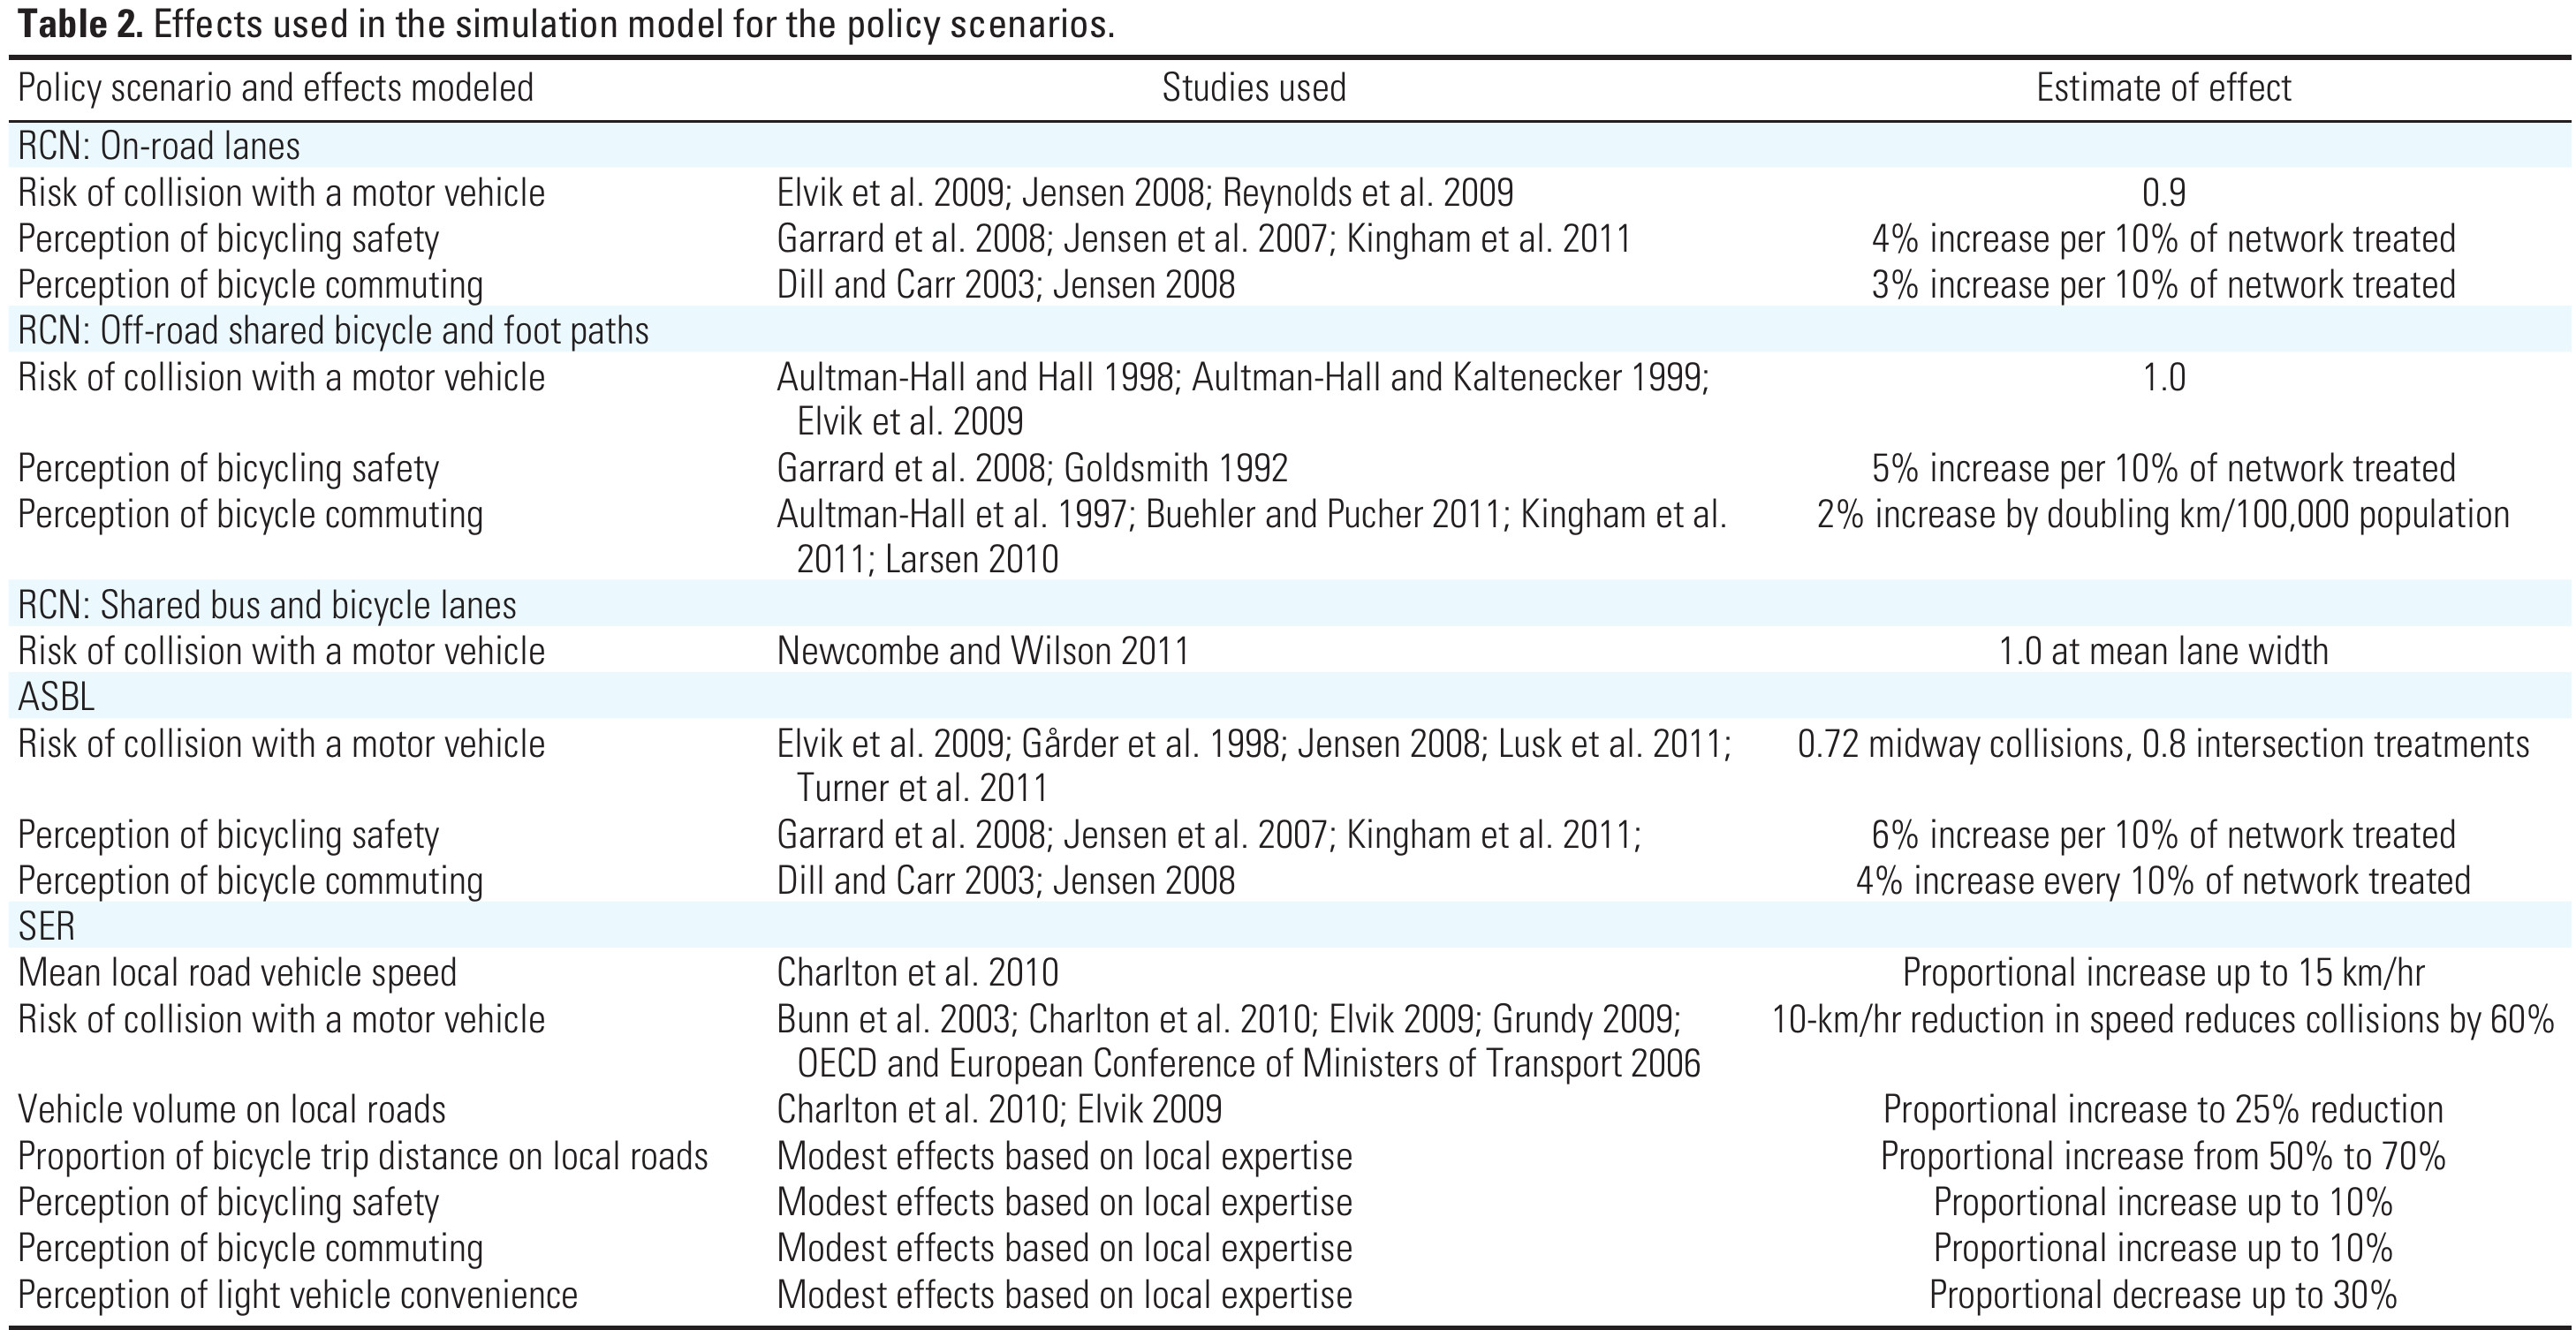
\includegraphics[width=\textwidth]{Macmillan-table-2.jpg}
\end{frame}

\subsection{Results}

\begin{frame}
  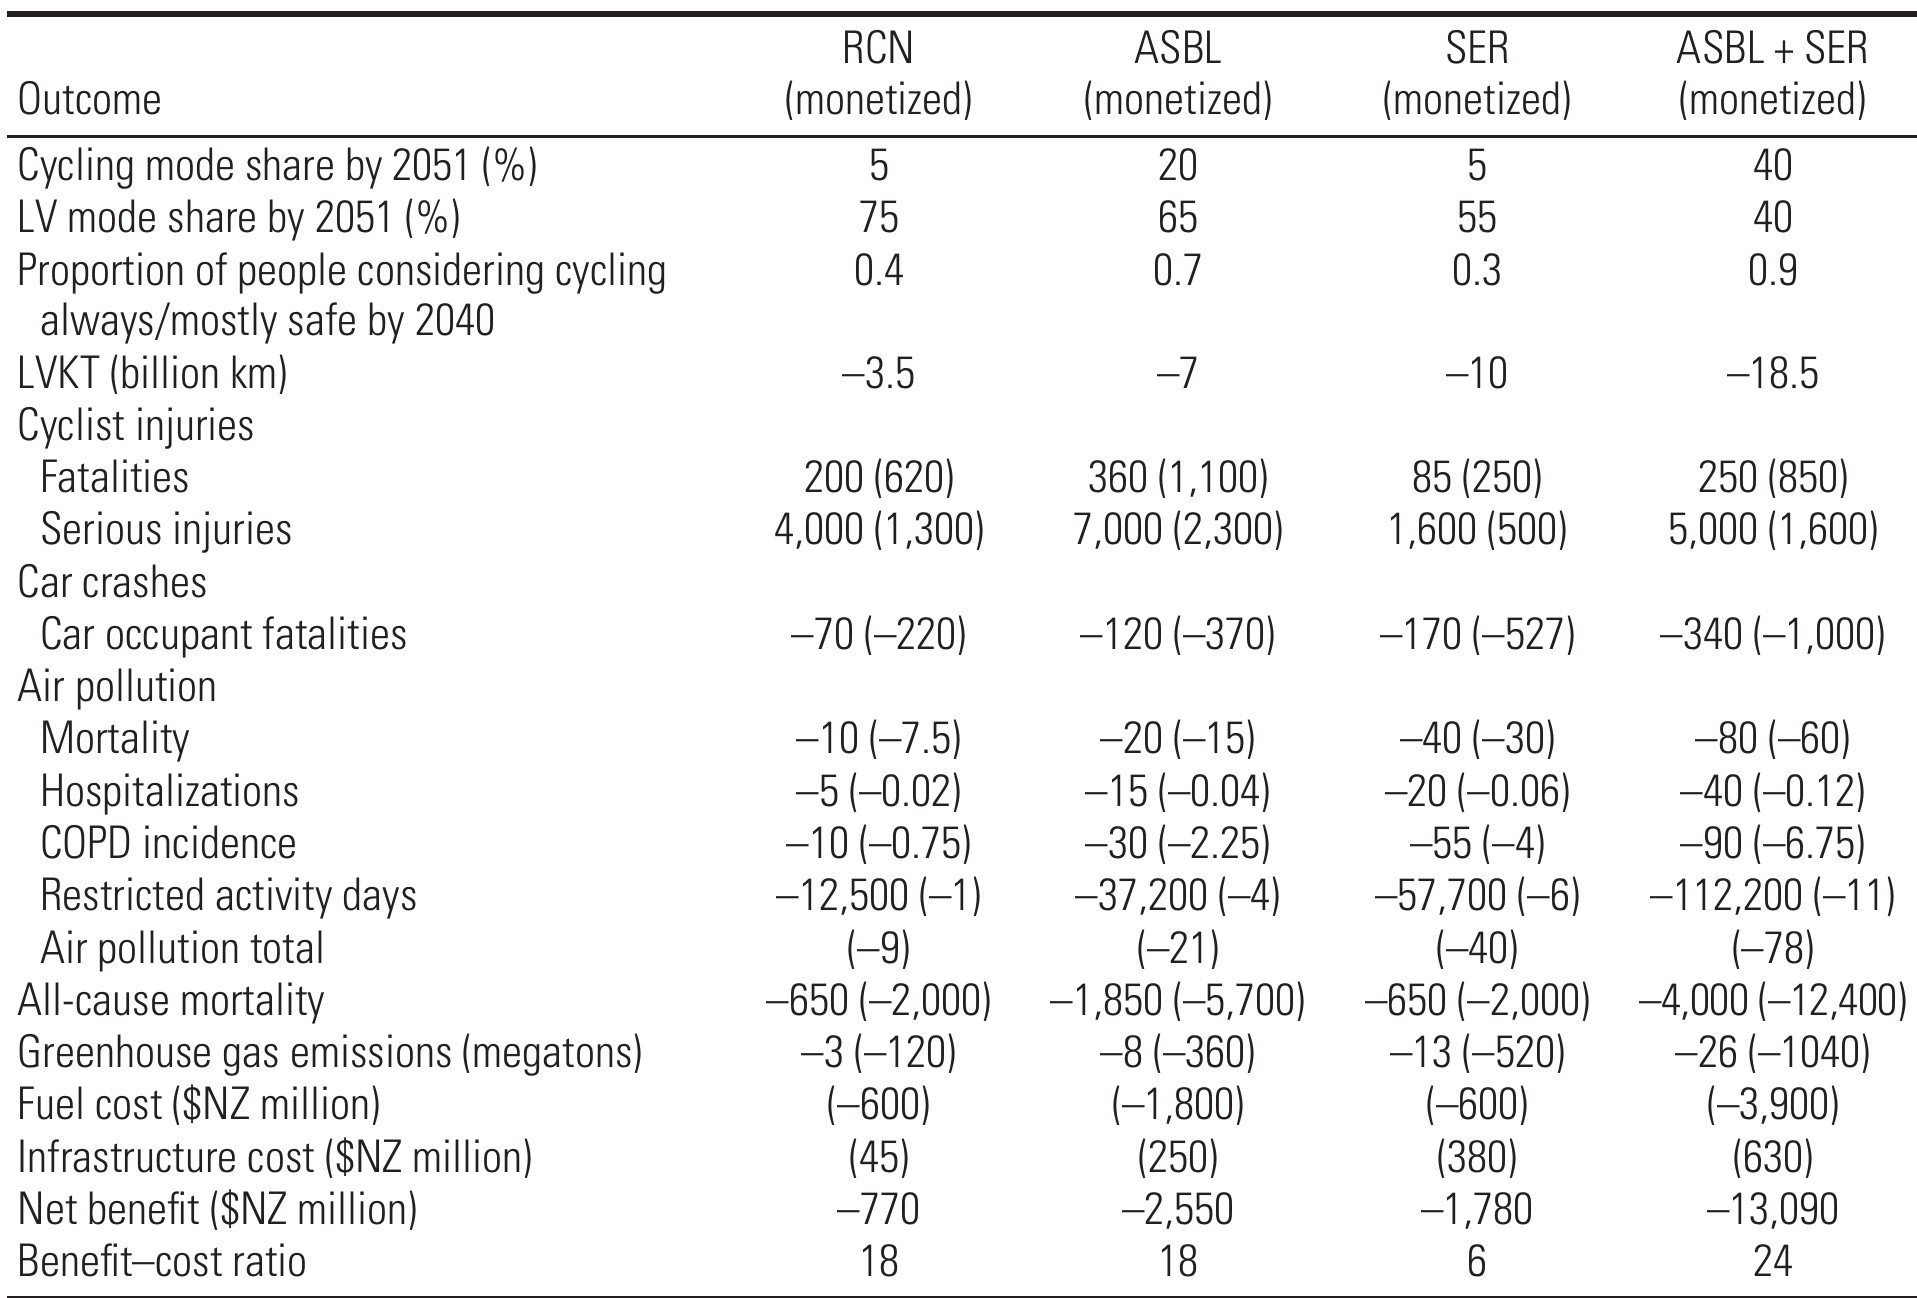
\includegraphics[width=\textwidth]{Macmillan-table-3.jpg}
\end{frame}

\begin{frame}
  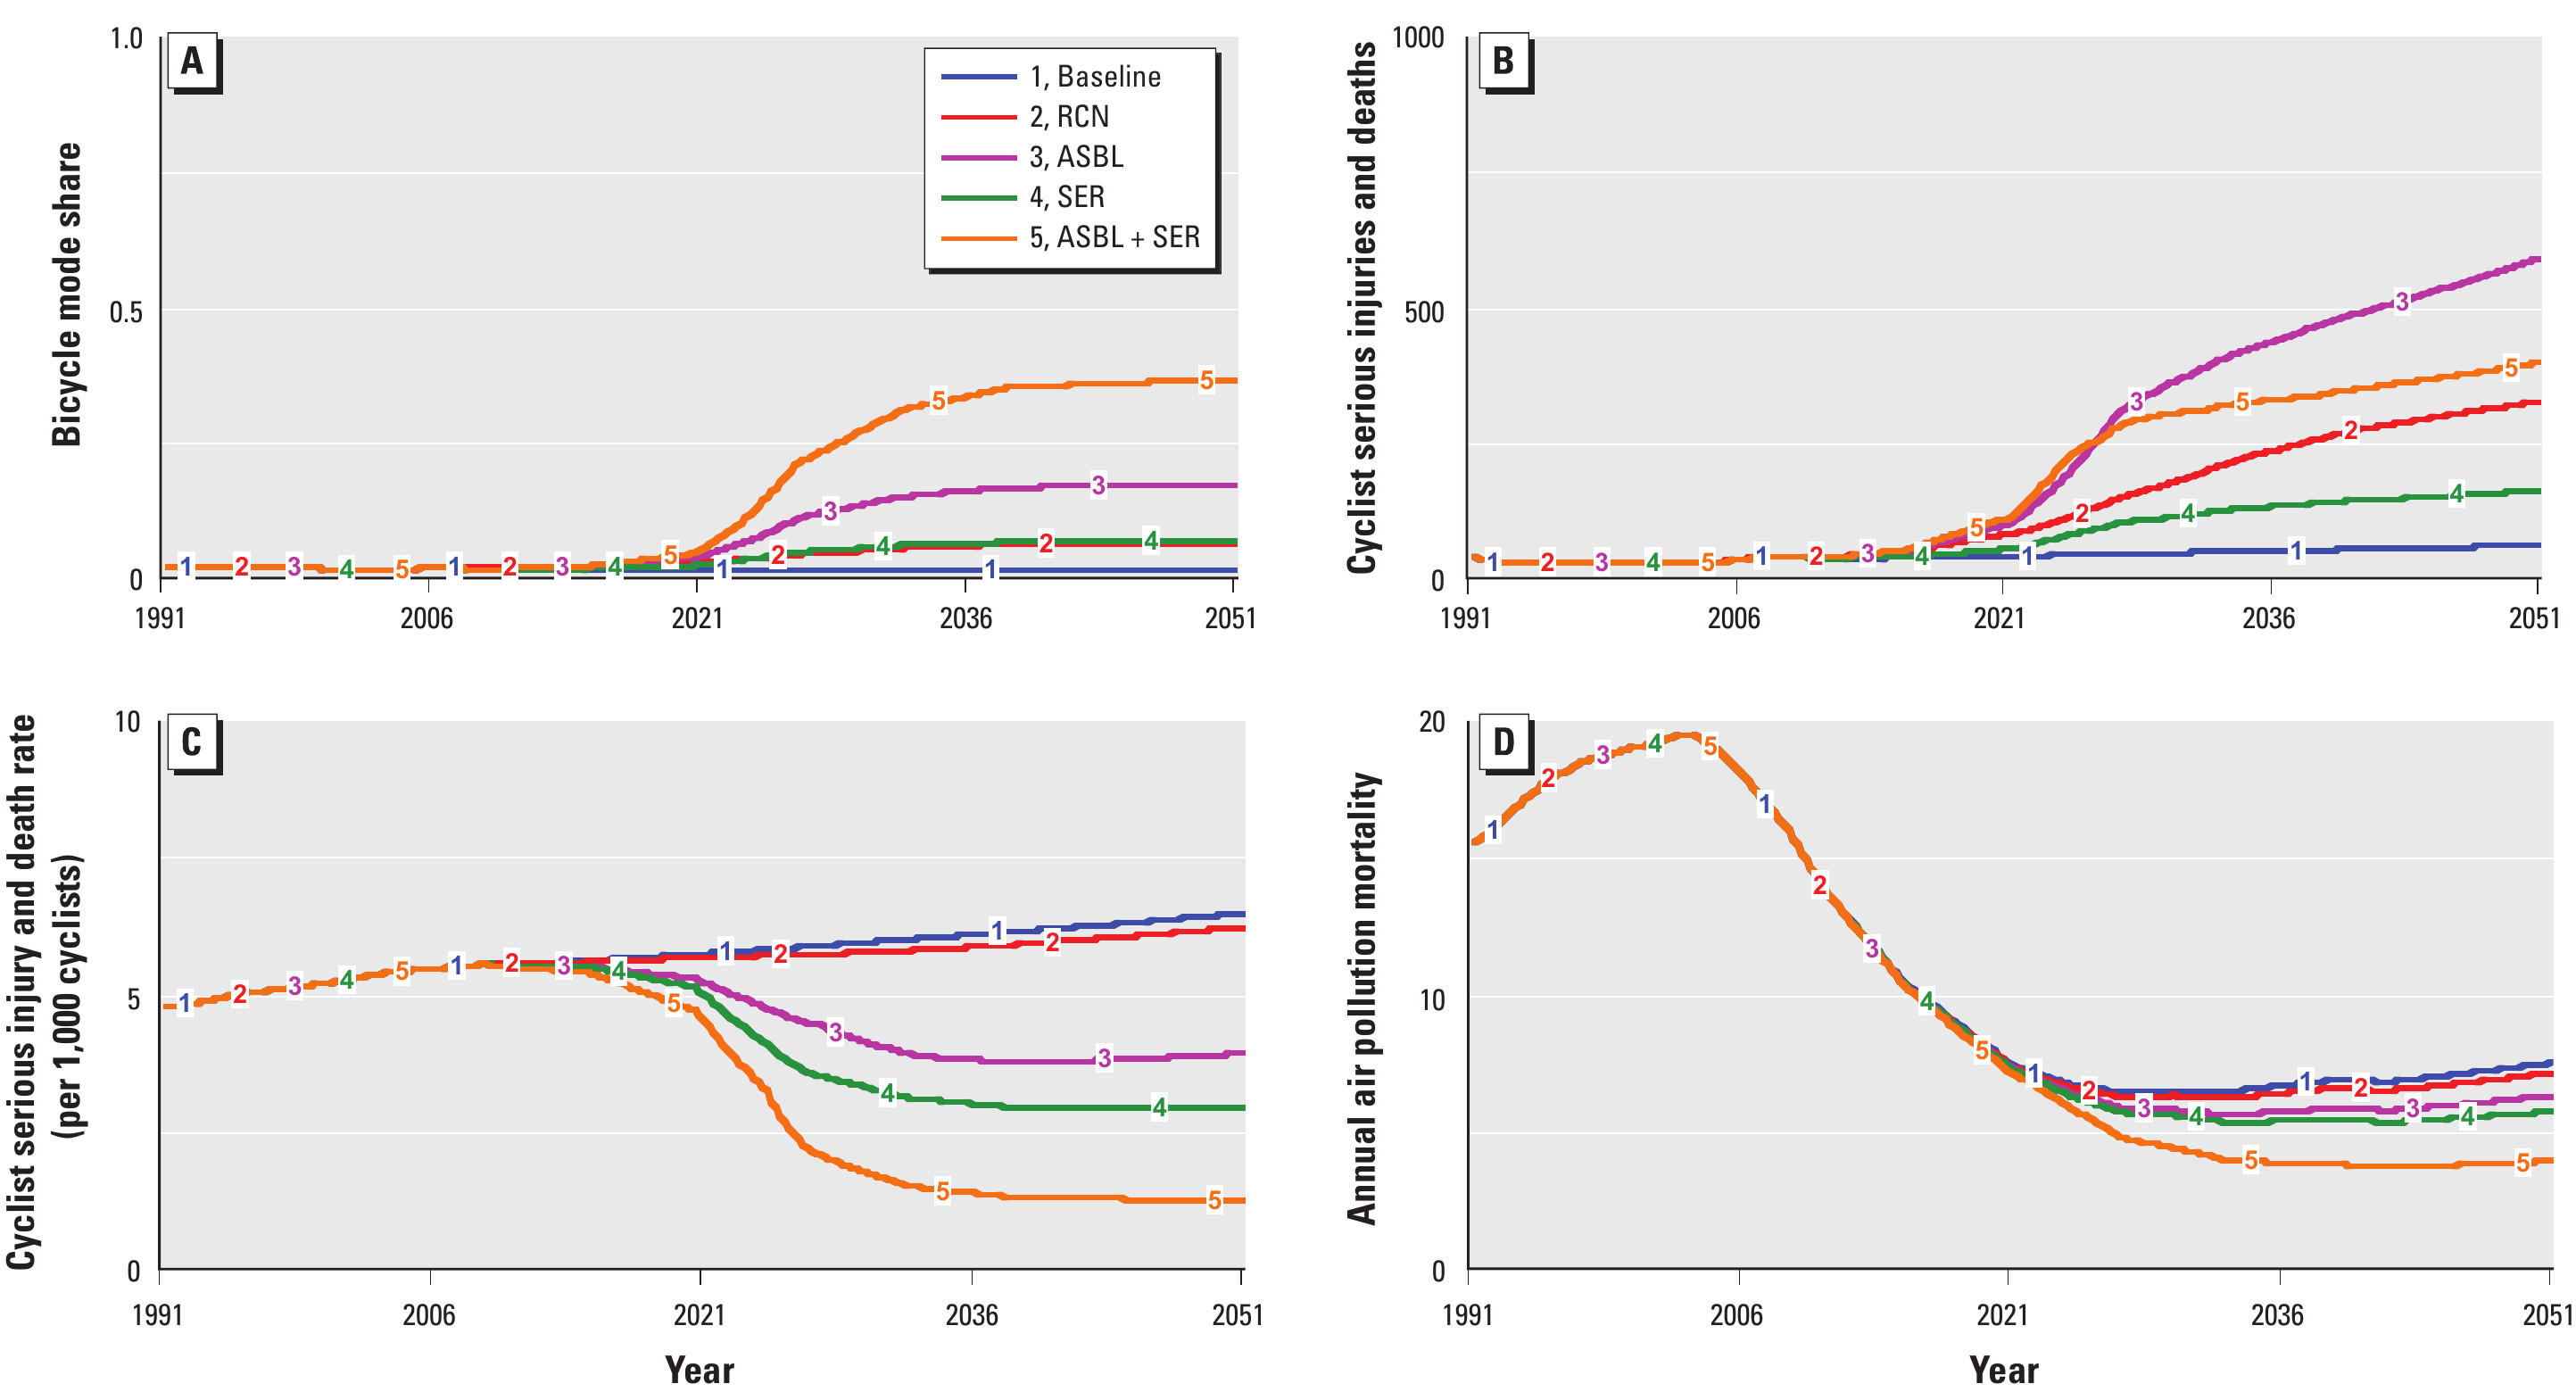
\includegraphics[width=\textwidth]{Macmillan-fig-2.jpg}
\end{frame}

\begin{frame}
  \frametitle{Results}
  \begin{itemize}
  \item No observed safety-in-numbers effect (so set a threshold?)
    \begin{itemize}
    \item cf.~Elvik and Goel, 2019 found regression coefficient $\approx 0.4$
    \end{itemize}
  \end{itemize}
\end{frame}


%%%%%%%%%%%%%%%%%%%%%%%%%%%%%%%%%%%%%%%%%%%%%%%%%%%%%%%%%%%%%%%%%

\section{Fagnant \& Kockelman 2014}

\subsection{Authors}

\begin{frame}
  \frametitle{The travel and environmental implications of shared autonomous vehicles}
  \begin{columns}
    \column{0.5\textwidth}
    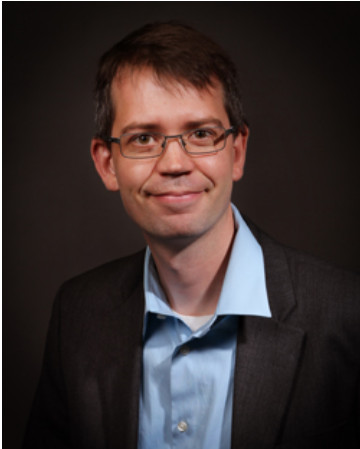
\includegraphics[height=0.3\textheight]{Fagnant.jpg}
    \begin{itemize}
    \item Daniel Fagnant
    \item (now) University of Utah, Dept of Civil \& Environmental Engineering
    \item PhD: University of Texas, Austin, 2014
    \end{itemize}
    \column{0.5\textwidth}
    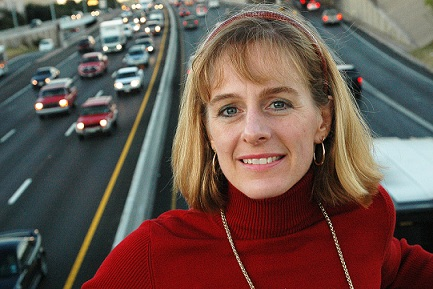
\includegraphics[height=0.3\textheight]{Kockelman.jpg}
    \begin{itemize}
    \item Kara Kockelman
    \item University of Texas, Austin, Dept of Civil, Architectural, Environmental Eng
    \item PhD: Berkeley, 1998
    \end{itemize}
  \end{columns}
  \vskip 3 mm
  Transportation Research Part C: emerging technologies. I.F. $\approx 6$
\end{frame}

\subsection{Why?}

\begin{frame}
  \frametitle{Why share cars?}
  \begin{itemize}
  \item More utility, less responsibility
  \item Reduce demand for parking
  \item Reduce parking-seeking congestion
  \item Autonomous vehicle safety
  \item Environmental benefits?
    \begin{itemize}
    \item Reduce trips by car?!
    \item Reduce parking surface area (e.g. from 14\%)
    \item Increase fleet turnover
    \item Reduce cold starts
    \item Embedded energy (reduce \# cars by factor of 9--12)
    \end{itemize}
  \end{itemize}
\end{frame}

\subsection{Model}

\begin{frame}
  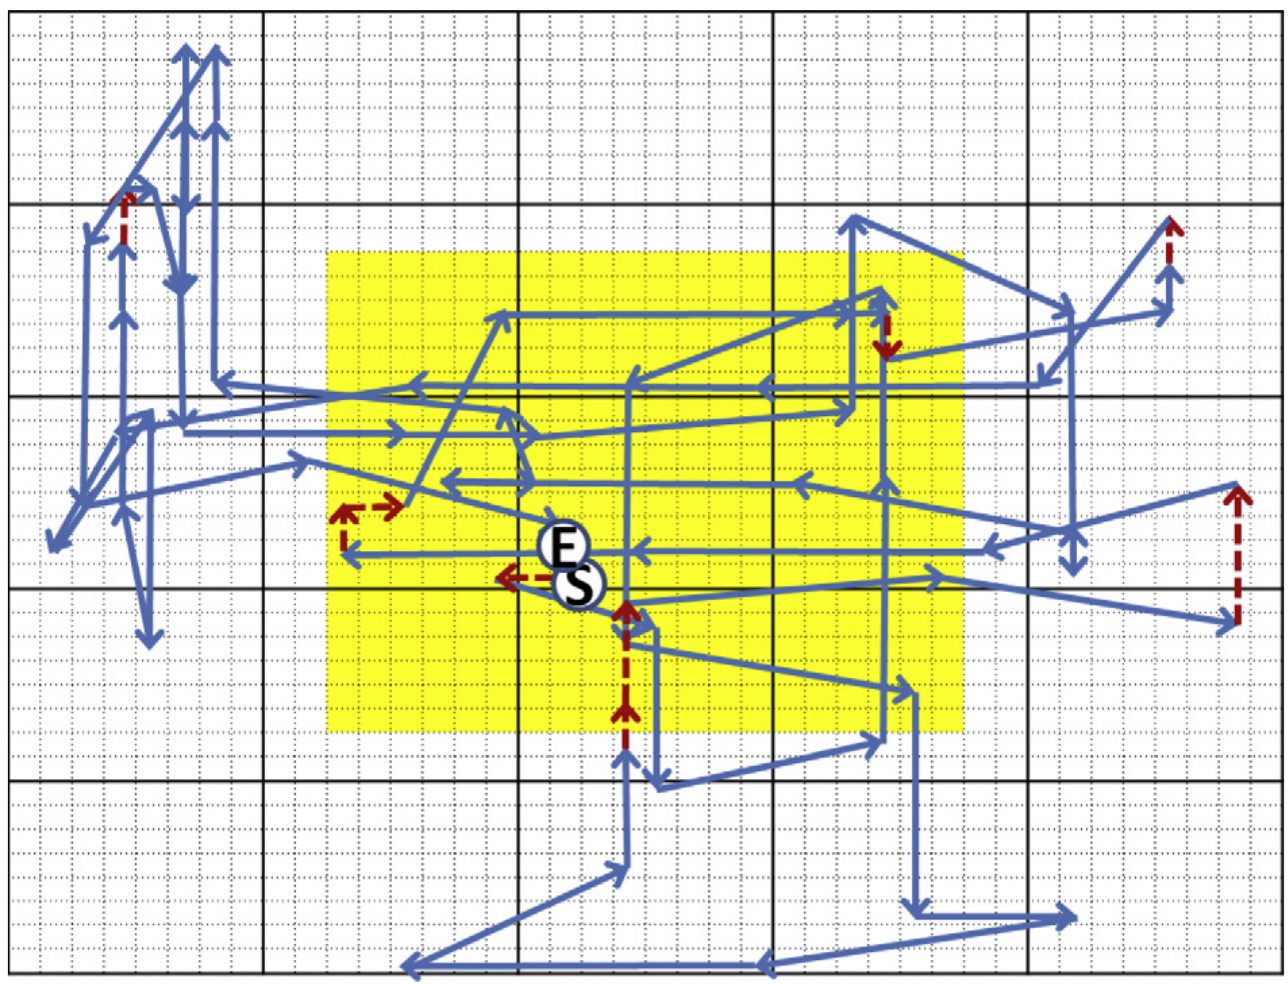
\includegraphics[height=\textheight]{Fagnant-fig-5.jpg}
\end{frame}

\begin{frame}
  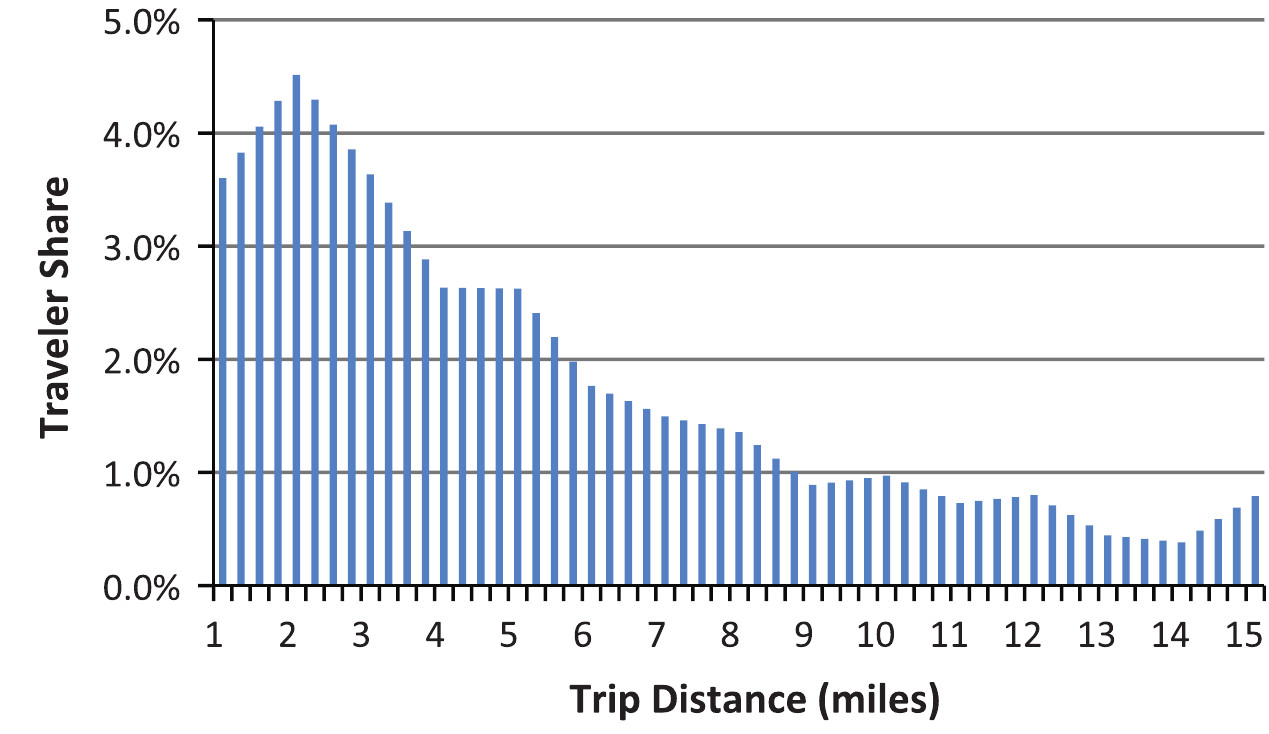
\includegraphics[width=\textwidth]{Fagnant-fig-1.jpg}
\end{frame}

\begin{frame}
  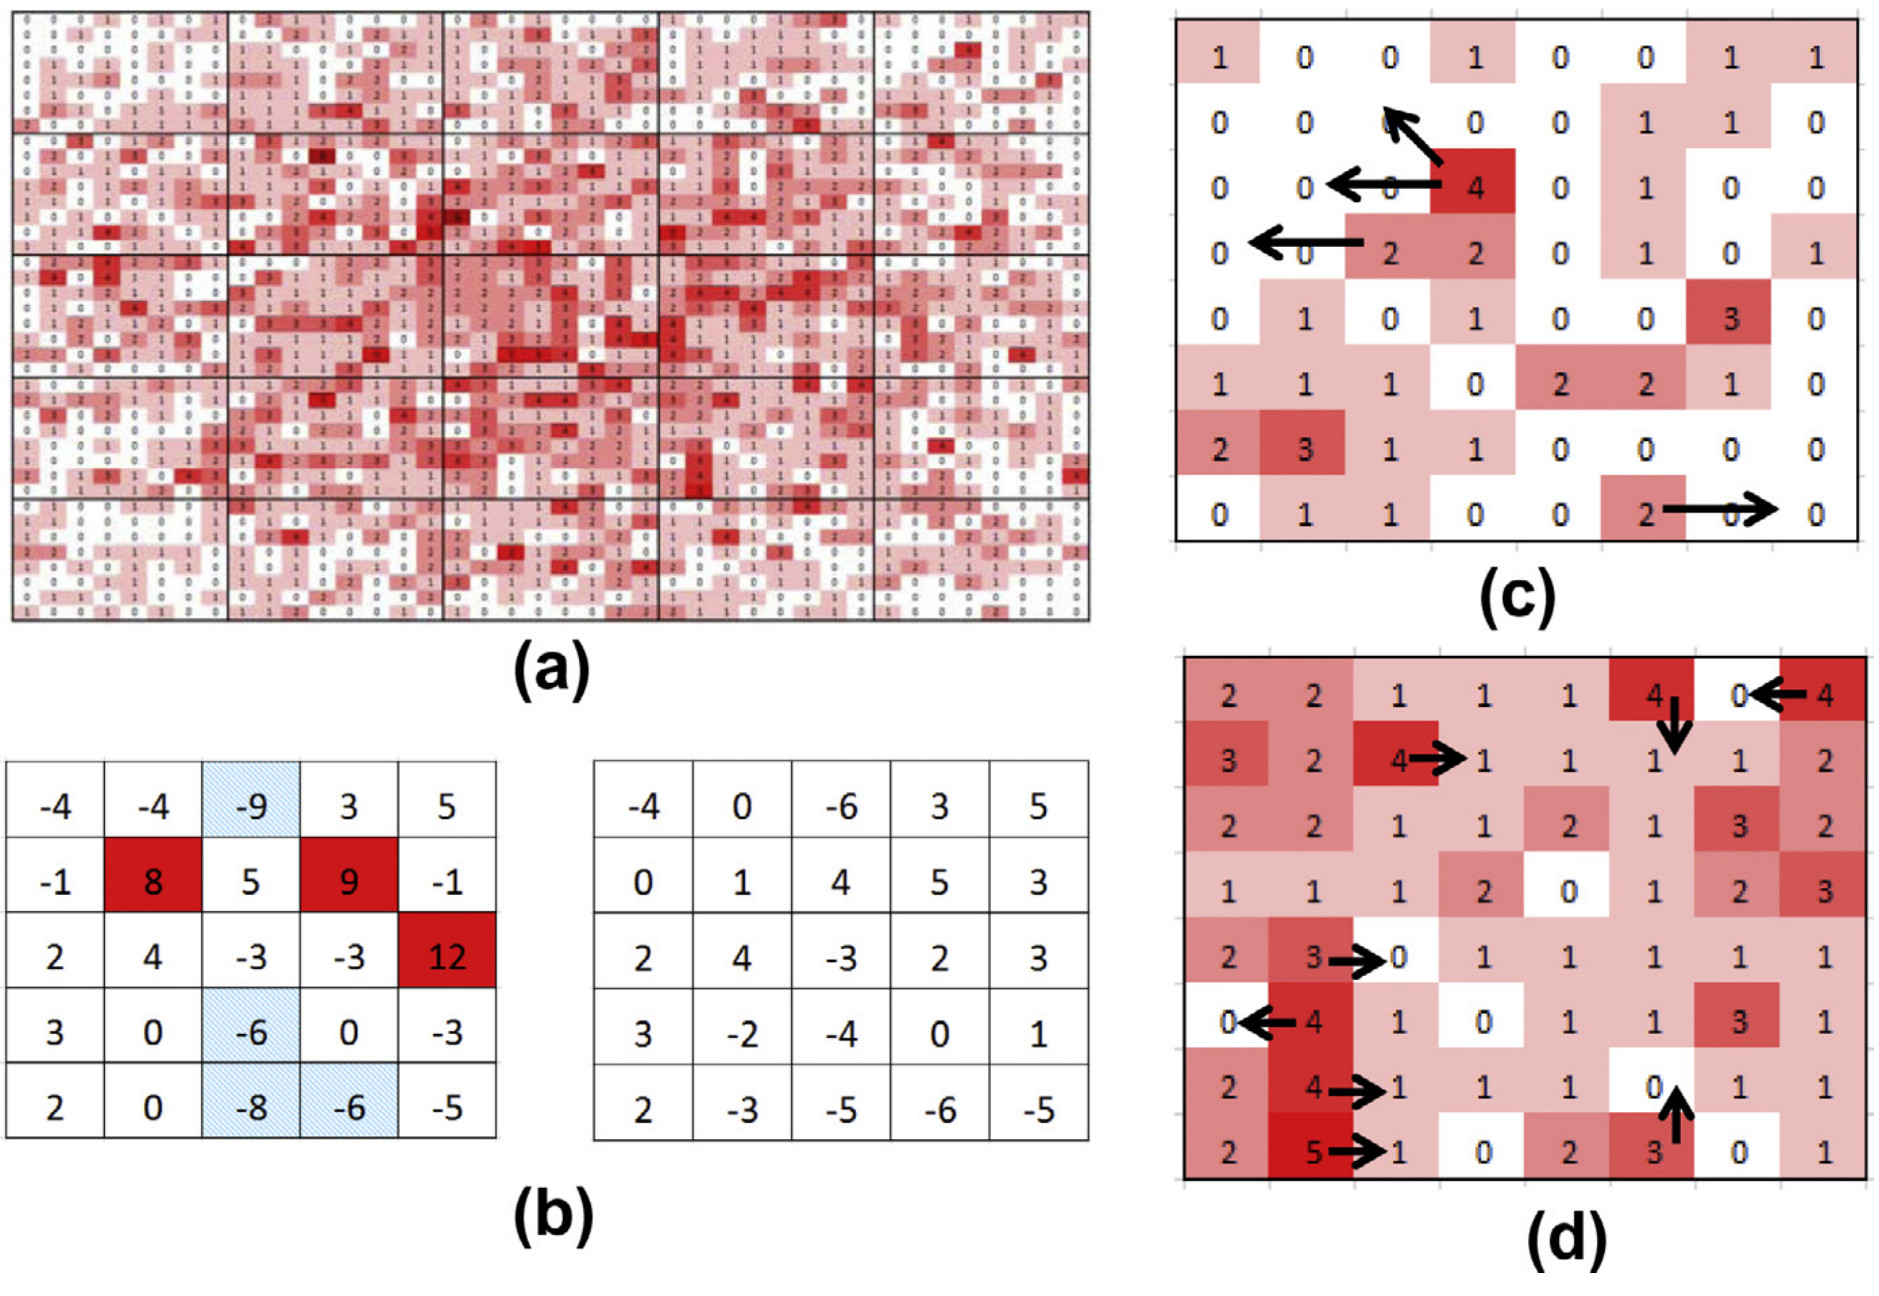
\includegraphics[width=\textwidth]{Fagnant-fig-4.jpg}
\end{frame}

\subsection{Results}

\begin{frame}
  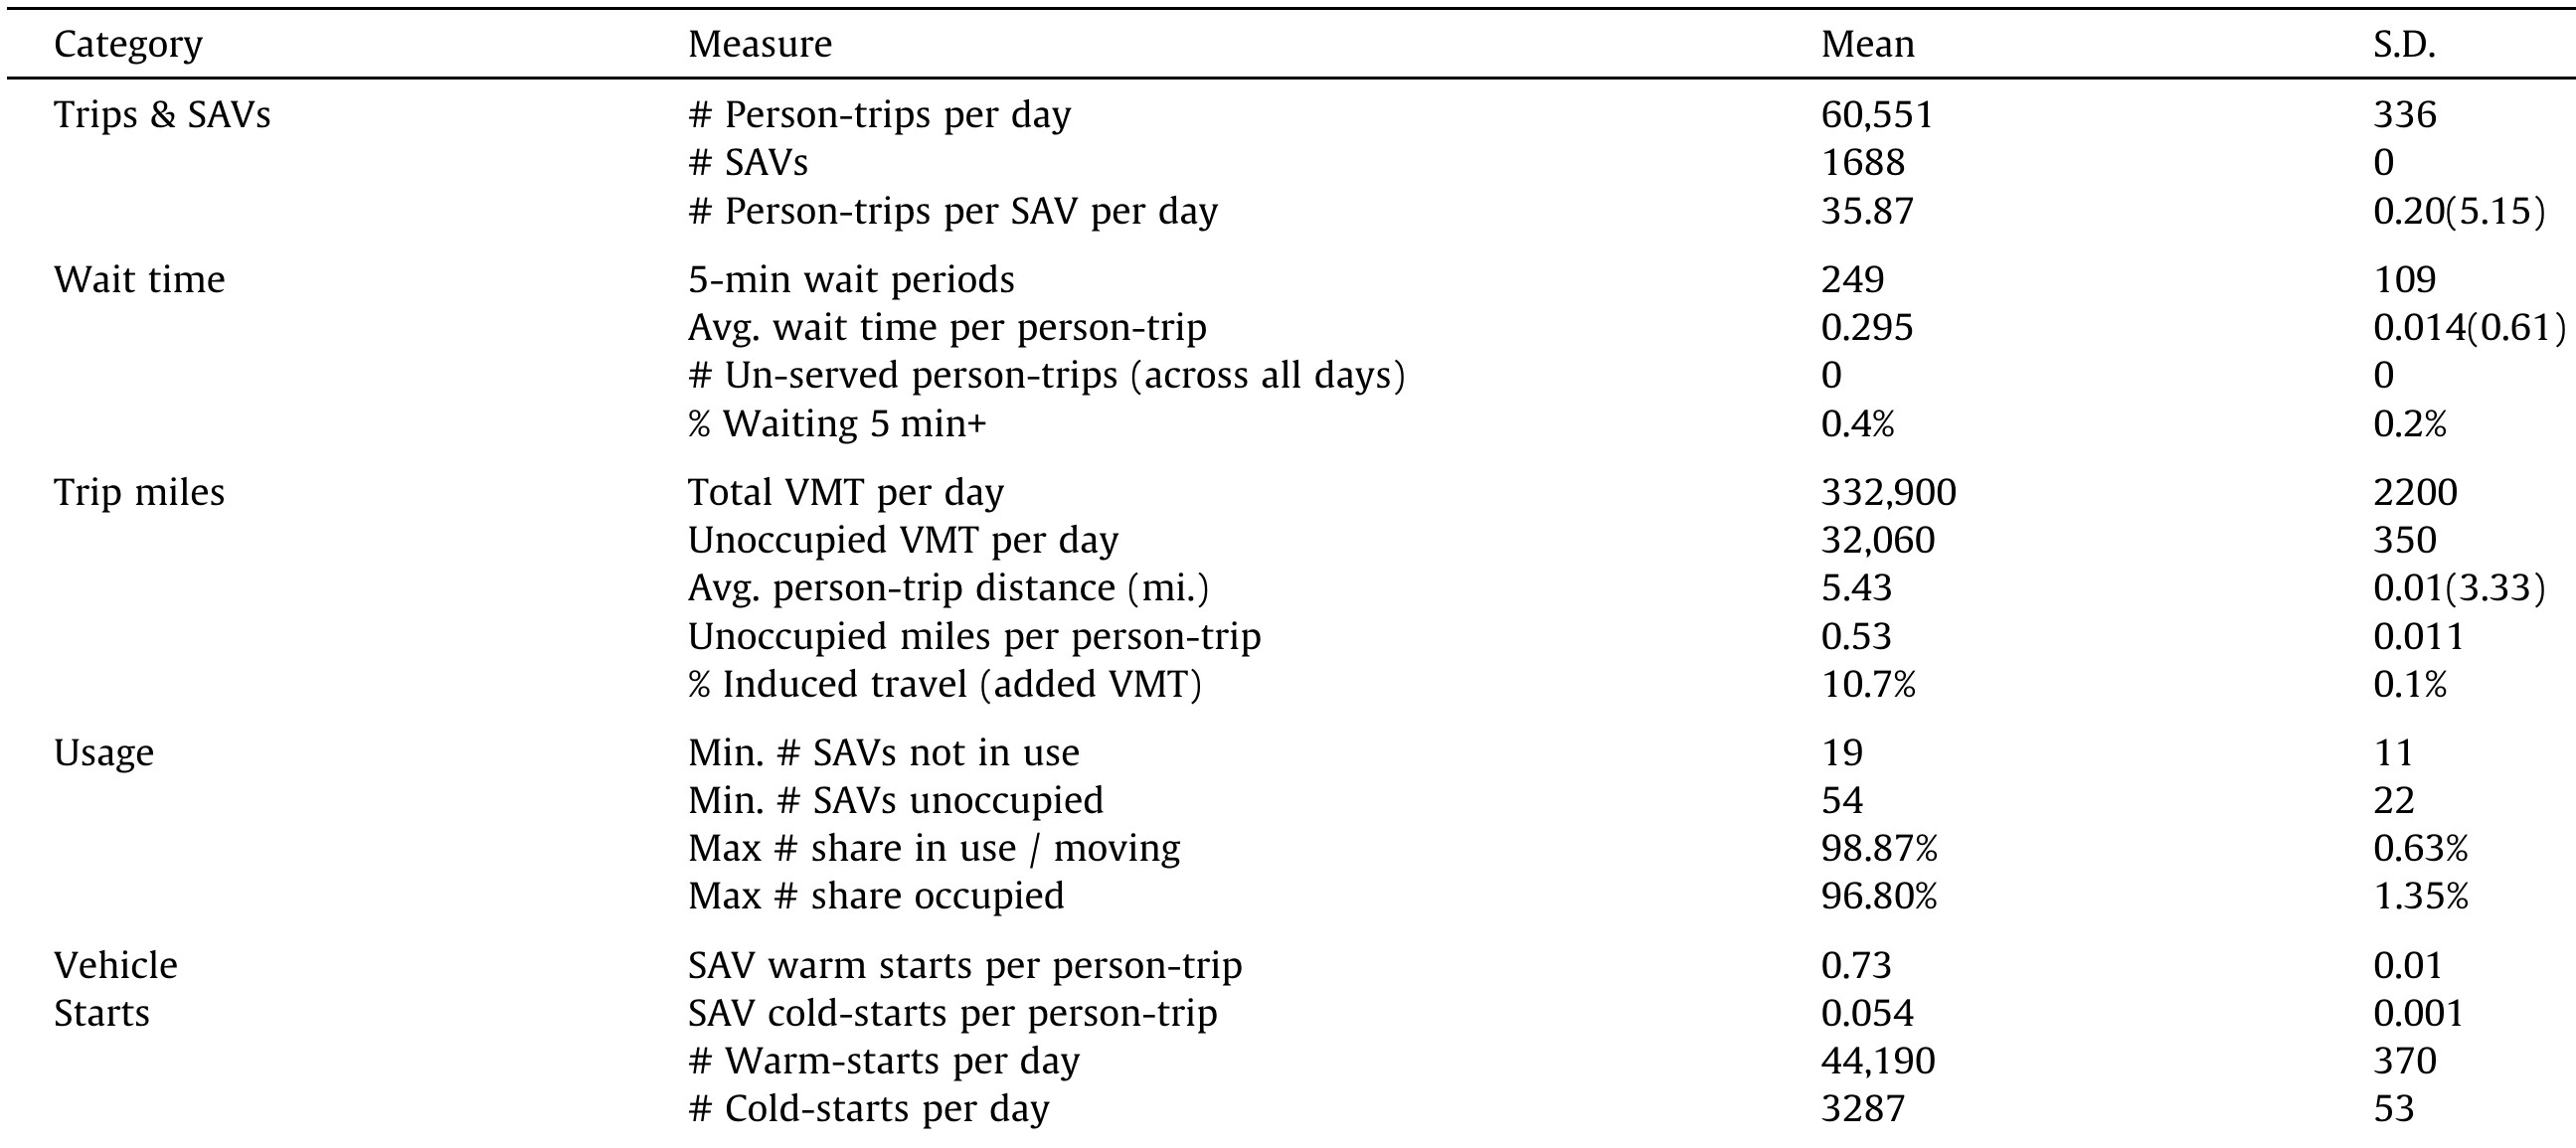
\includegraphics[width=\textwidth]{Fagnant-table-2.jpg}
\end{frame}

\begin{frame}
  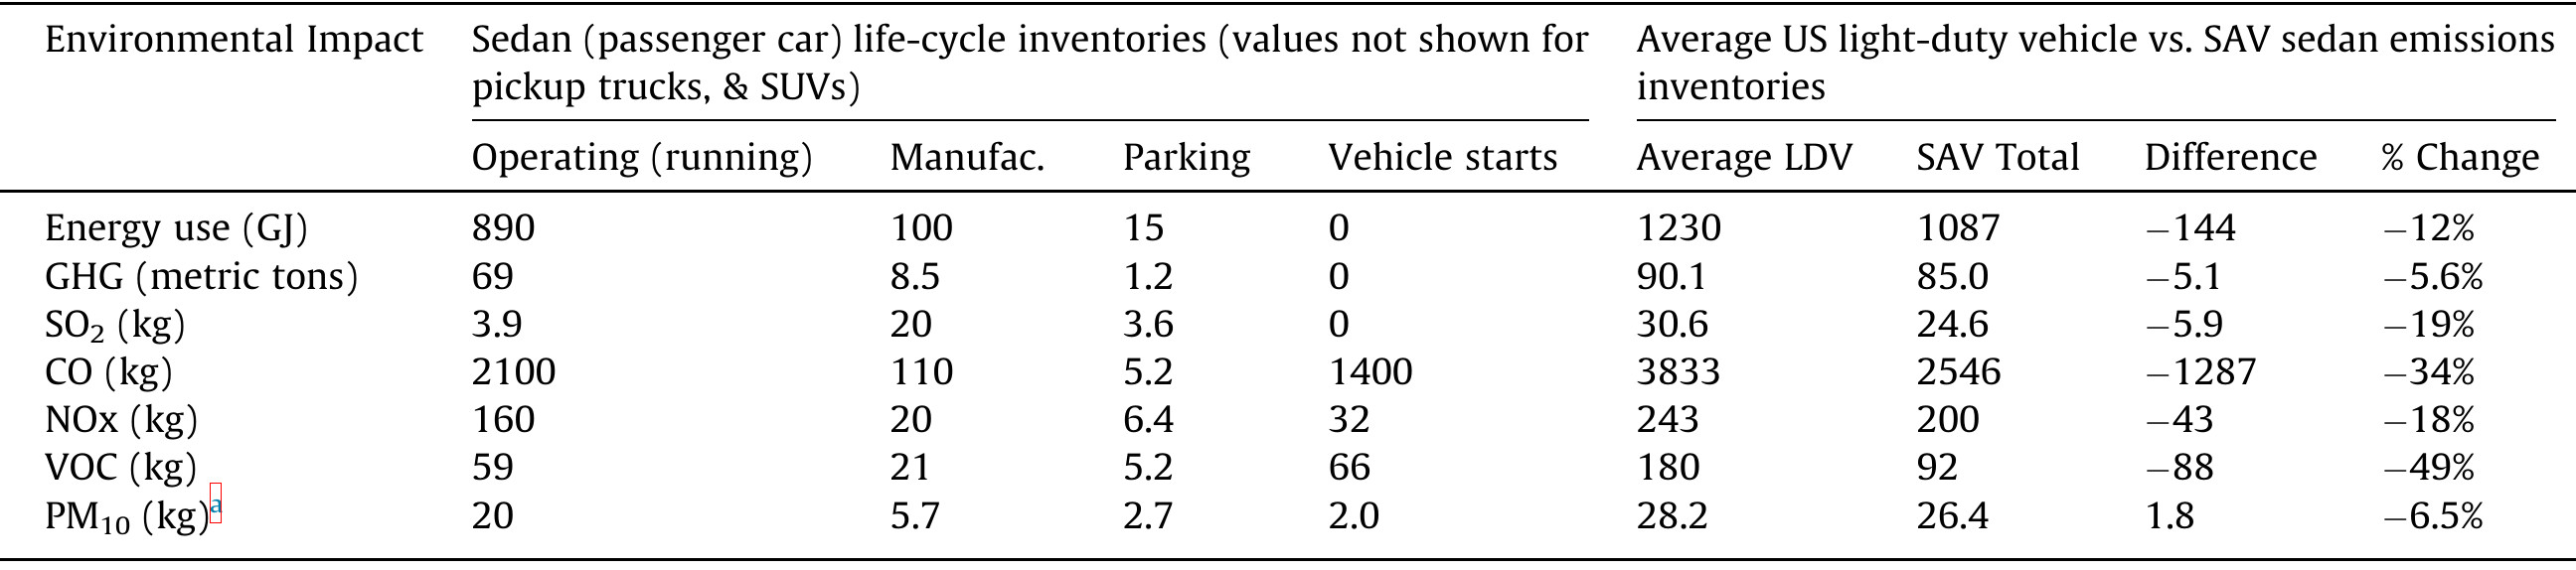
\includegraphics[width=\textwidth]{Fagnant-table-3.jpg}
\end{frame}

\begin{frame}
  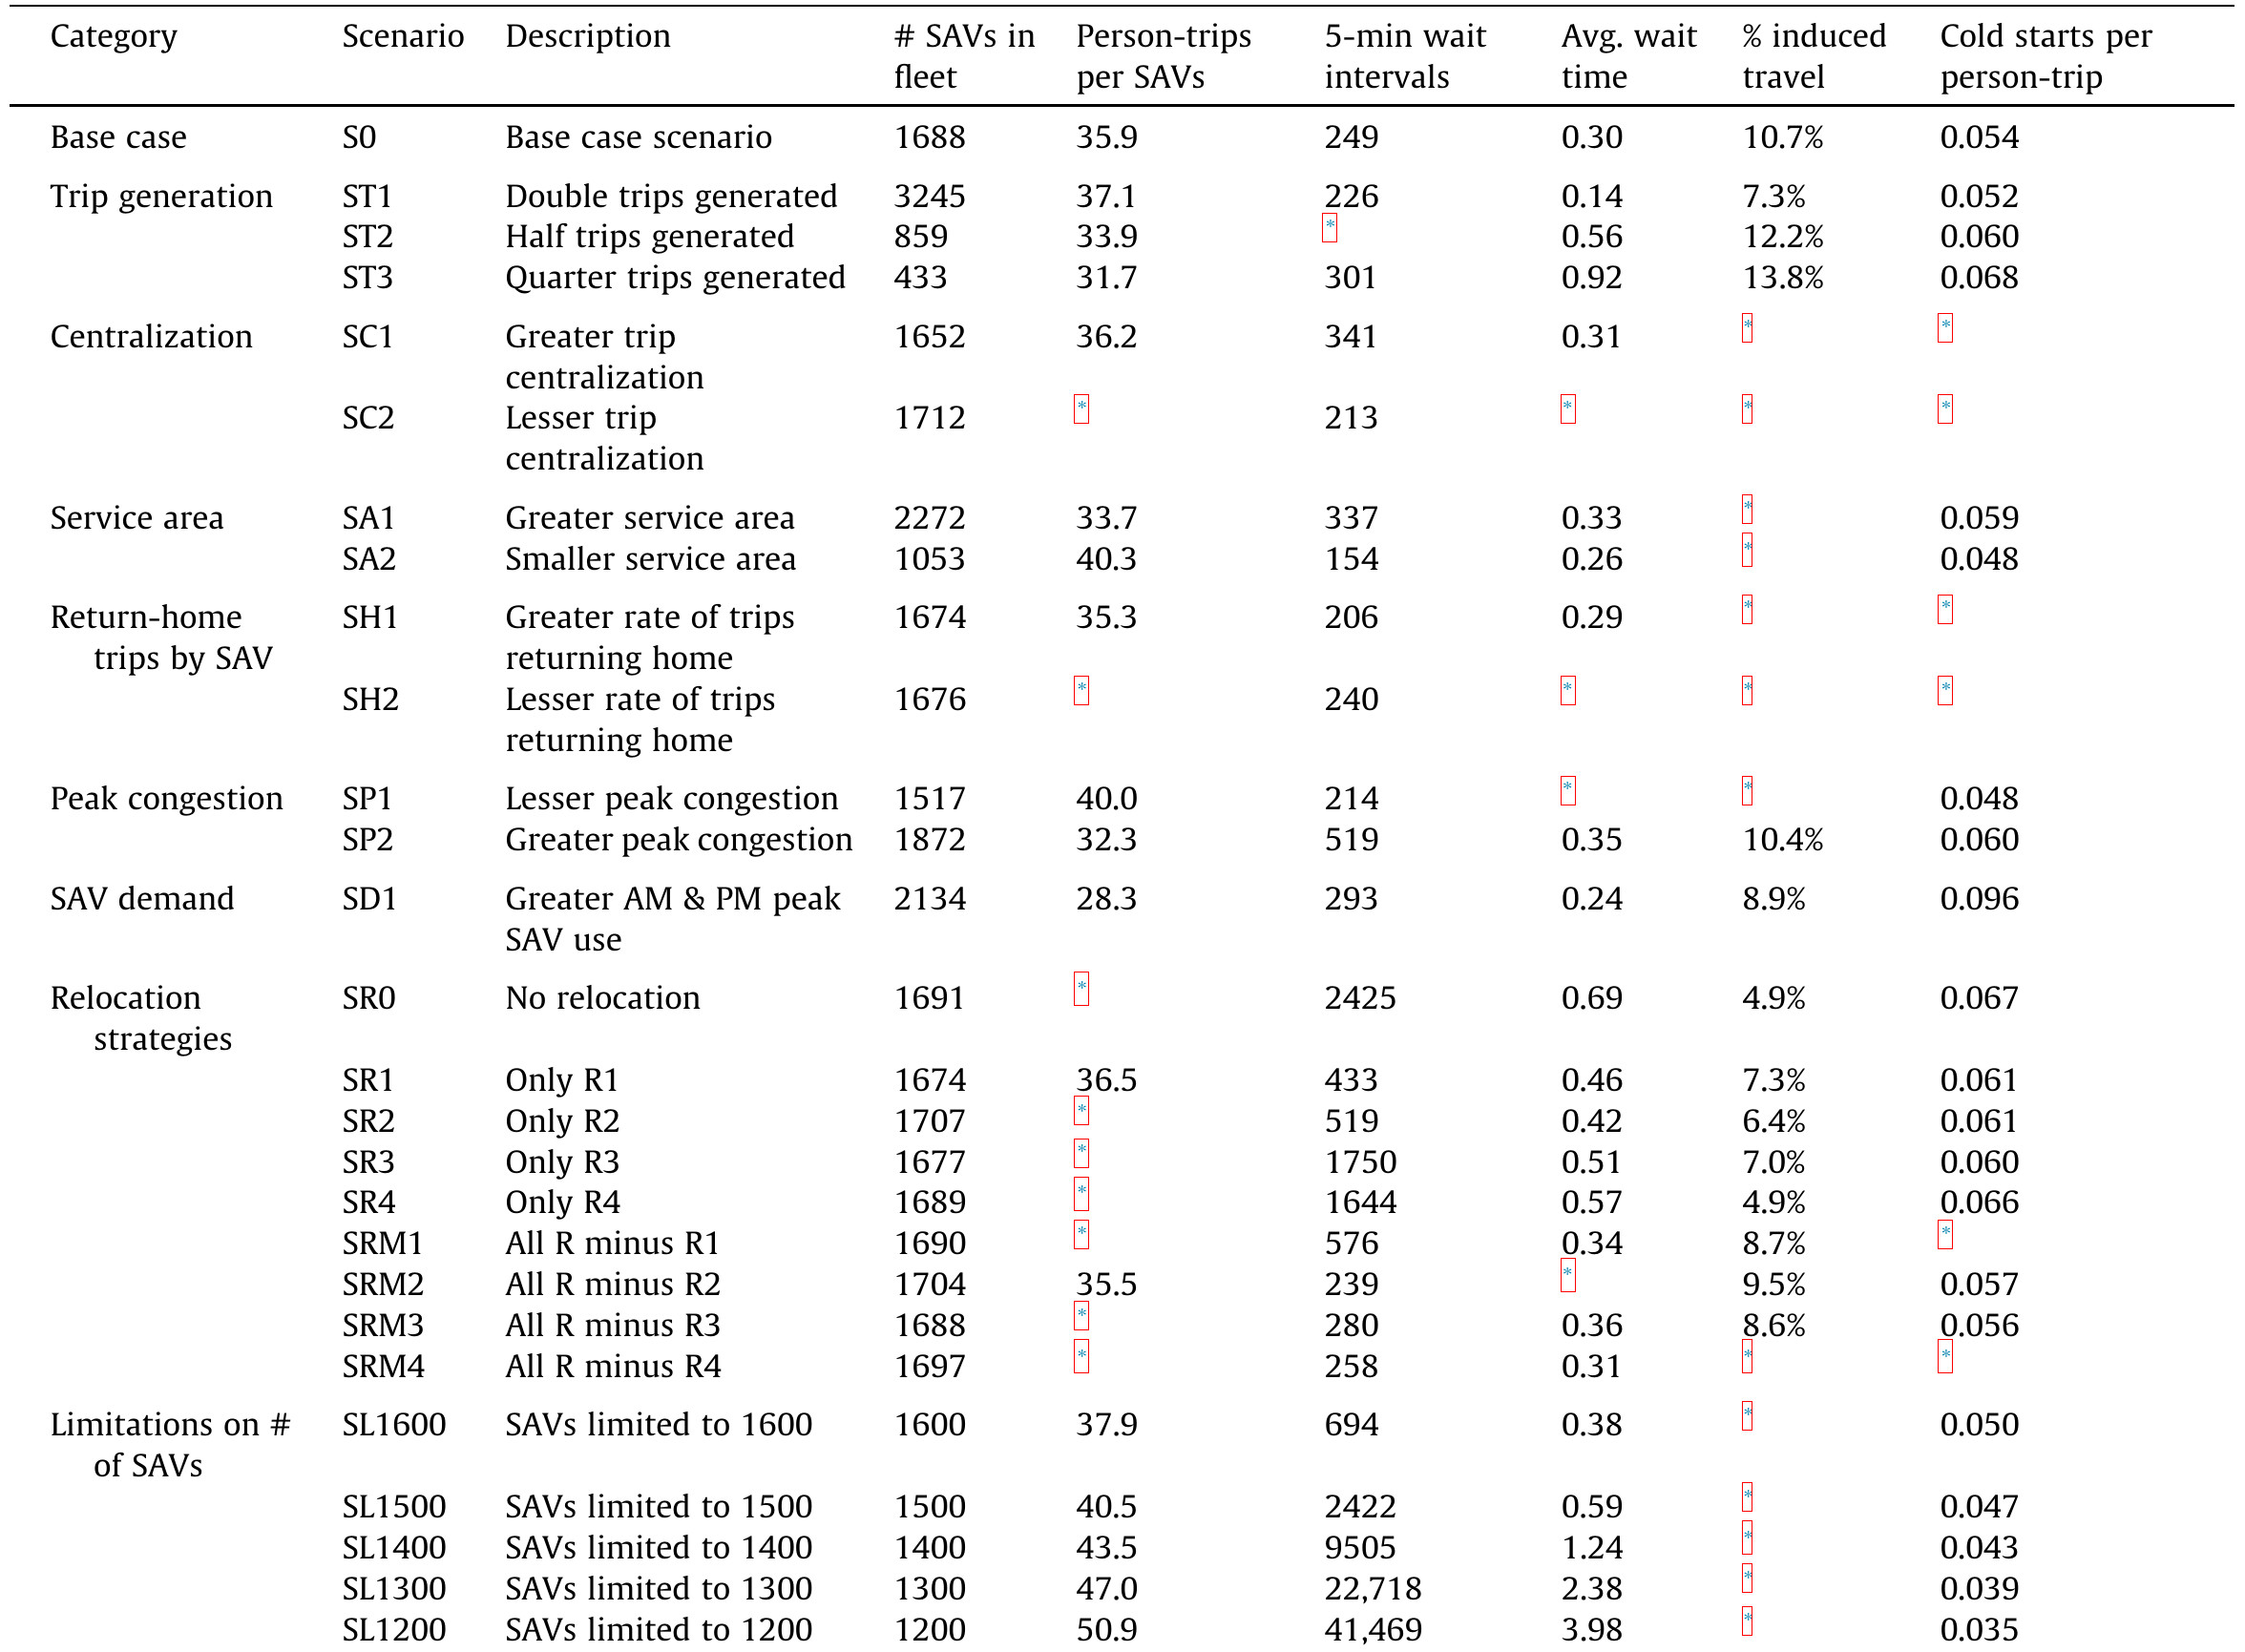
\includegraphics[width=\textwidth]{Fagnant-table-4.jpg}
\end{frame}

\begin{frame}
  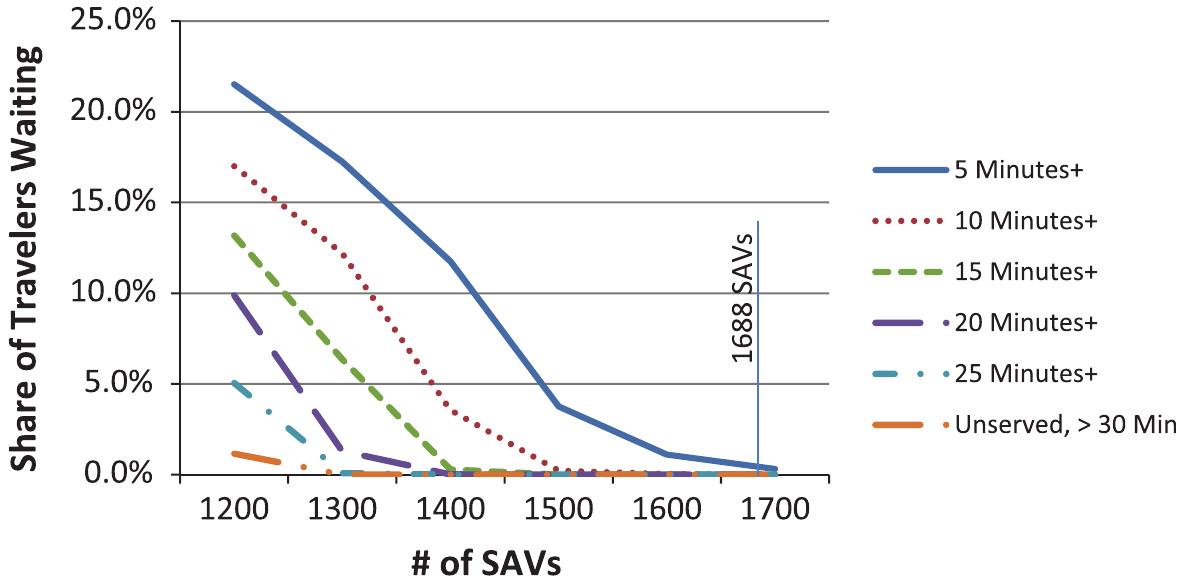
\includegraphics[width=\textwidth]{Fagnant-fig-6.jpg}
\end{frame}

\subsection{Discuss}

\begin{frame}
  \frametitle{Weird\dots}
  \begin{itemize}
  \item Demand is exogenous?
    \begin{itemize}
    \item Shaheen and Cohen (2013) estimate 27\% reduction in trips
    \item Seems at odds with lots of research on induced demand\dots
      \begin{itemize}
      \item Uber+Lyft generating huge increase in trips, pollution, congestion, accidents
      \end{itemize}
    \end{itemize}
  \item Relocation strategy?
  \item Would delay shift to electric vehicles?
  \end{itemize}
\end{frame}




%%%%%%%%%%%%%%%%%%%%%%%%%%%%%%%%%%%%%%%%%%%%%%%%%%%%%%%%%%%%%%%%%%%

\section{Struben \& Sterman 2006}

\begin{frame}
  \frametitle{Transition challenges for alternative fuel vehicle and transportation systems}
  \begin{columns}
    \column{0.5\textwidth}
    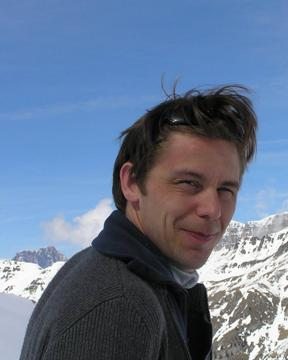
\includegraphics[height=0.3\textheight]{JeroenStruben.jpeg}
    \begin{itemize}
    \item Jeroen Struben
    \item (now) McGill University, System Dynamics
    \item PhD: MIT 2006
    \end{itemize}
    \column{0.5\textwidth}
    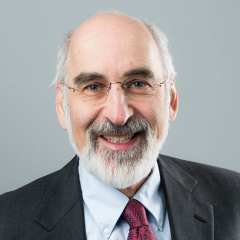
\includegraphics[height=0.3\textheight]{Sterman.png}
    \begin{itemize}
    \item John D Sterman
    \item PhD: MIT Sloan, 1982
    \item Wrote the book.
    \item Lots of fancy awards and stuff\dots
    \end{itemize}
  \end{columns}
  \vskip 3 mm
  Environment and Planning B (urban analytics): I.F.~$\lesssim 3$
\end{frame}

\subsection{Why?}


\begin{frame}
  \frametitle{Why?}
  Adoption of alternative-fuel vehicles (AFV) is driven by:
  \begin{itemize}
  \item Advertising
  \item Word of mouth from owners
  \item Gossip from non-owners
  \item Feature parity
  \item Fueling infrastructure (chicken-and-egg)
  \end{itemize}
  Main result: adoption governed by critical-mass threshold
\end{frame}

\subsection{Model}

\begin{frame}
  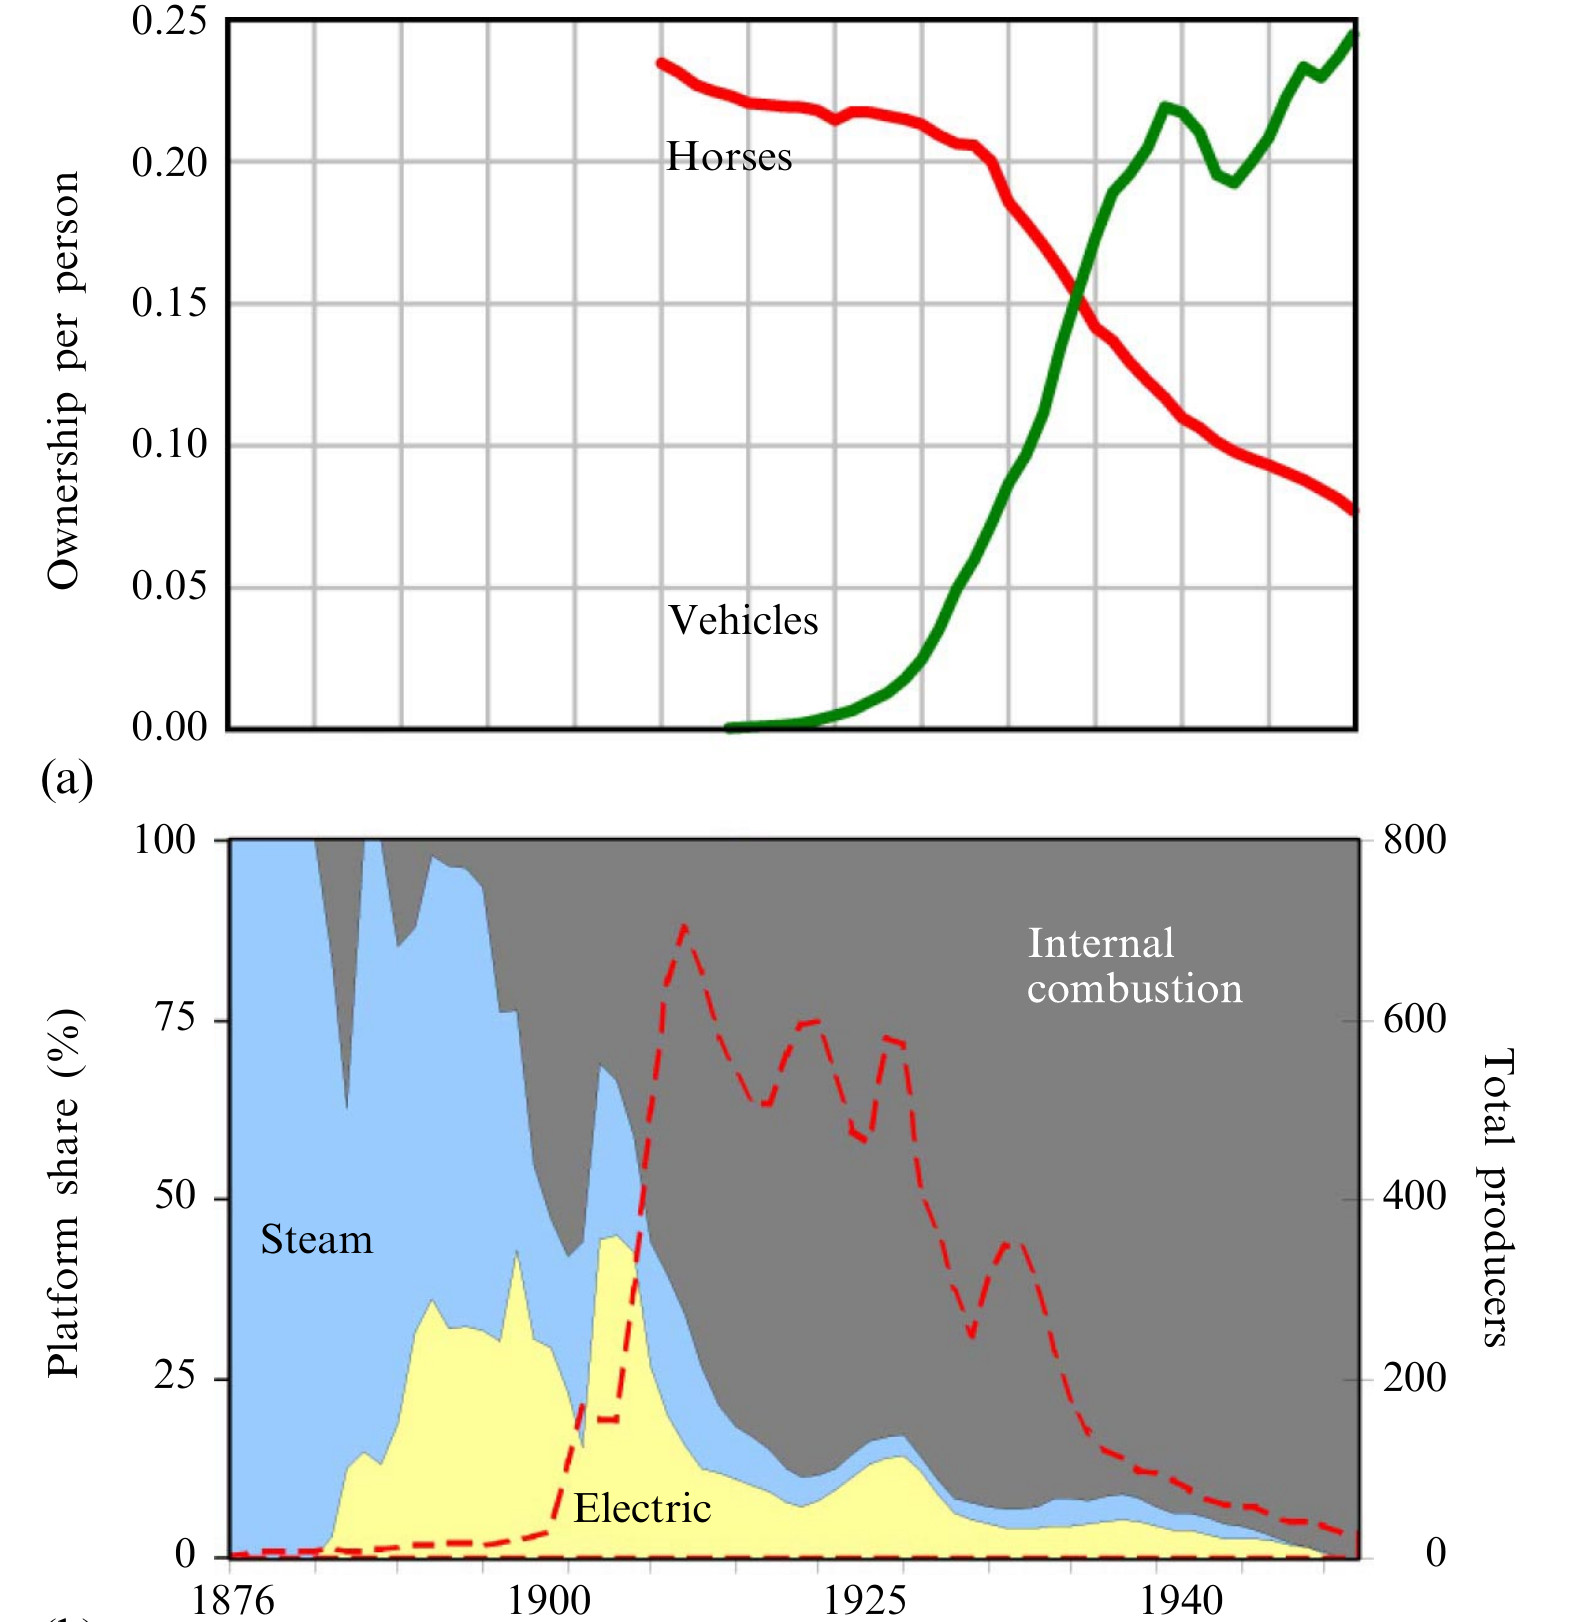
\includegraphics[height=\textheight]{Sterman-fig-1.jpg}
\end{frame}
    
\begin{frame}
  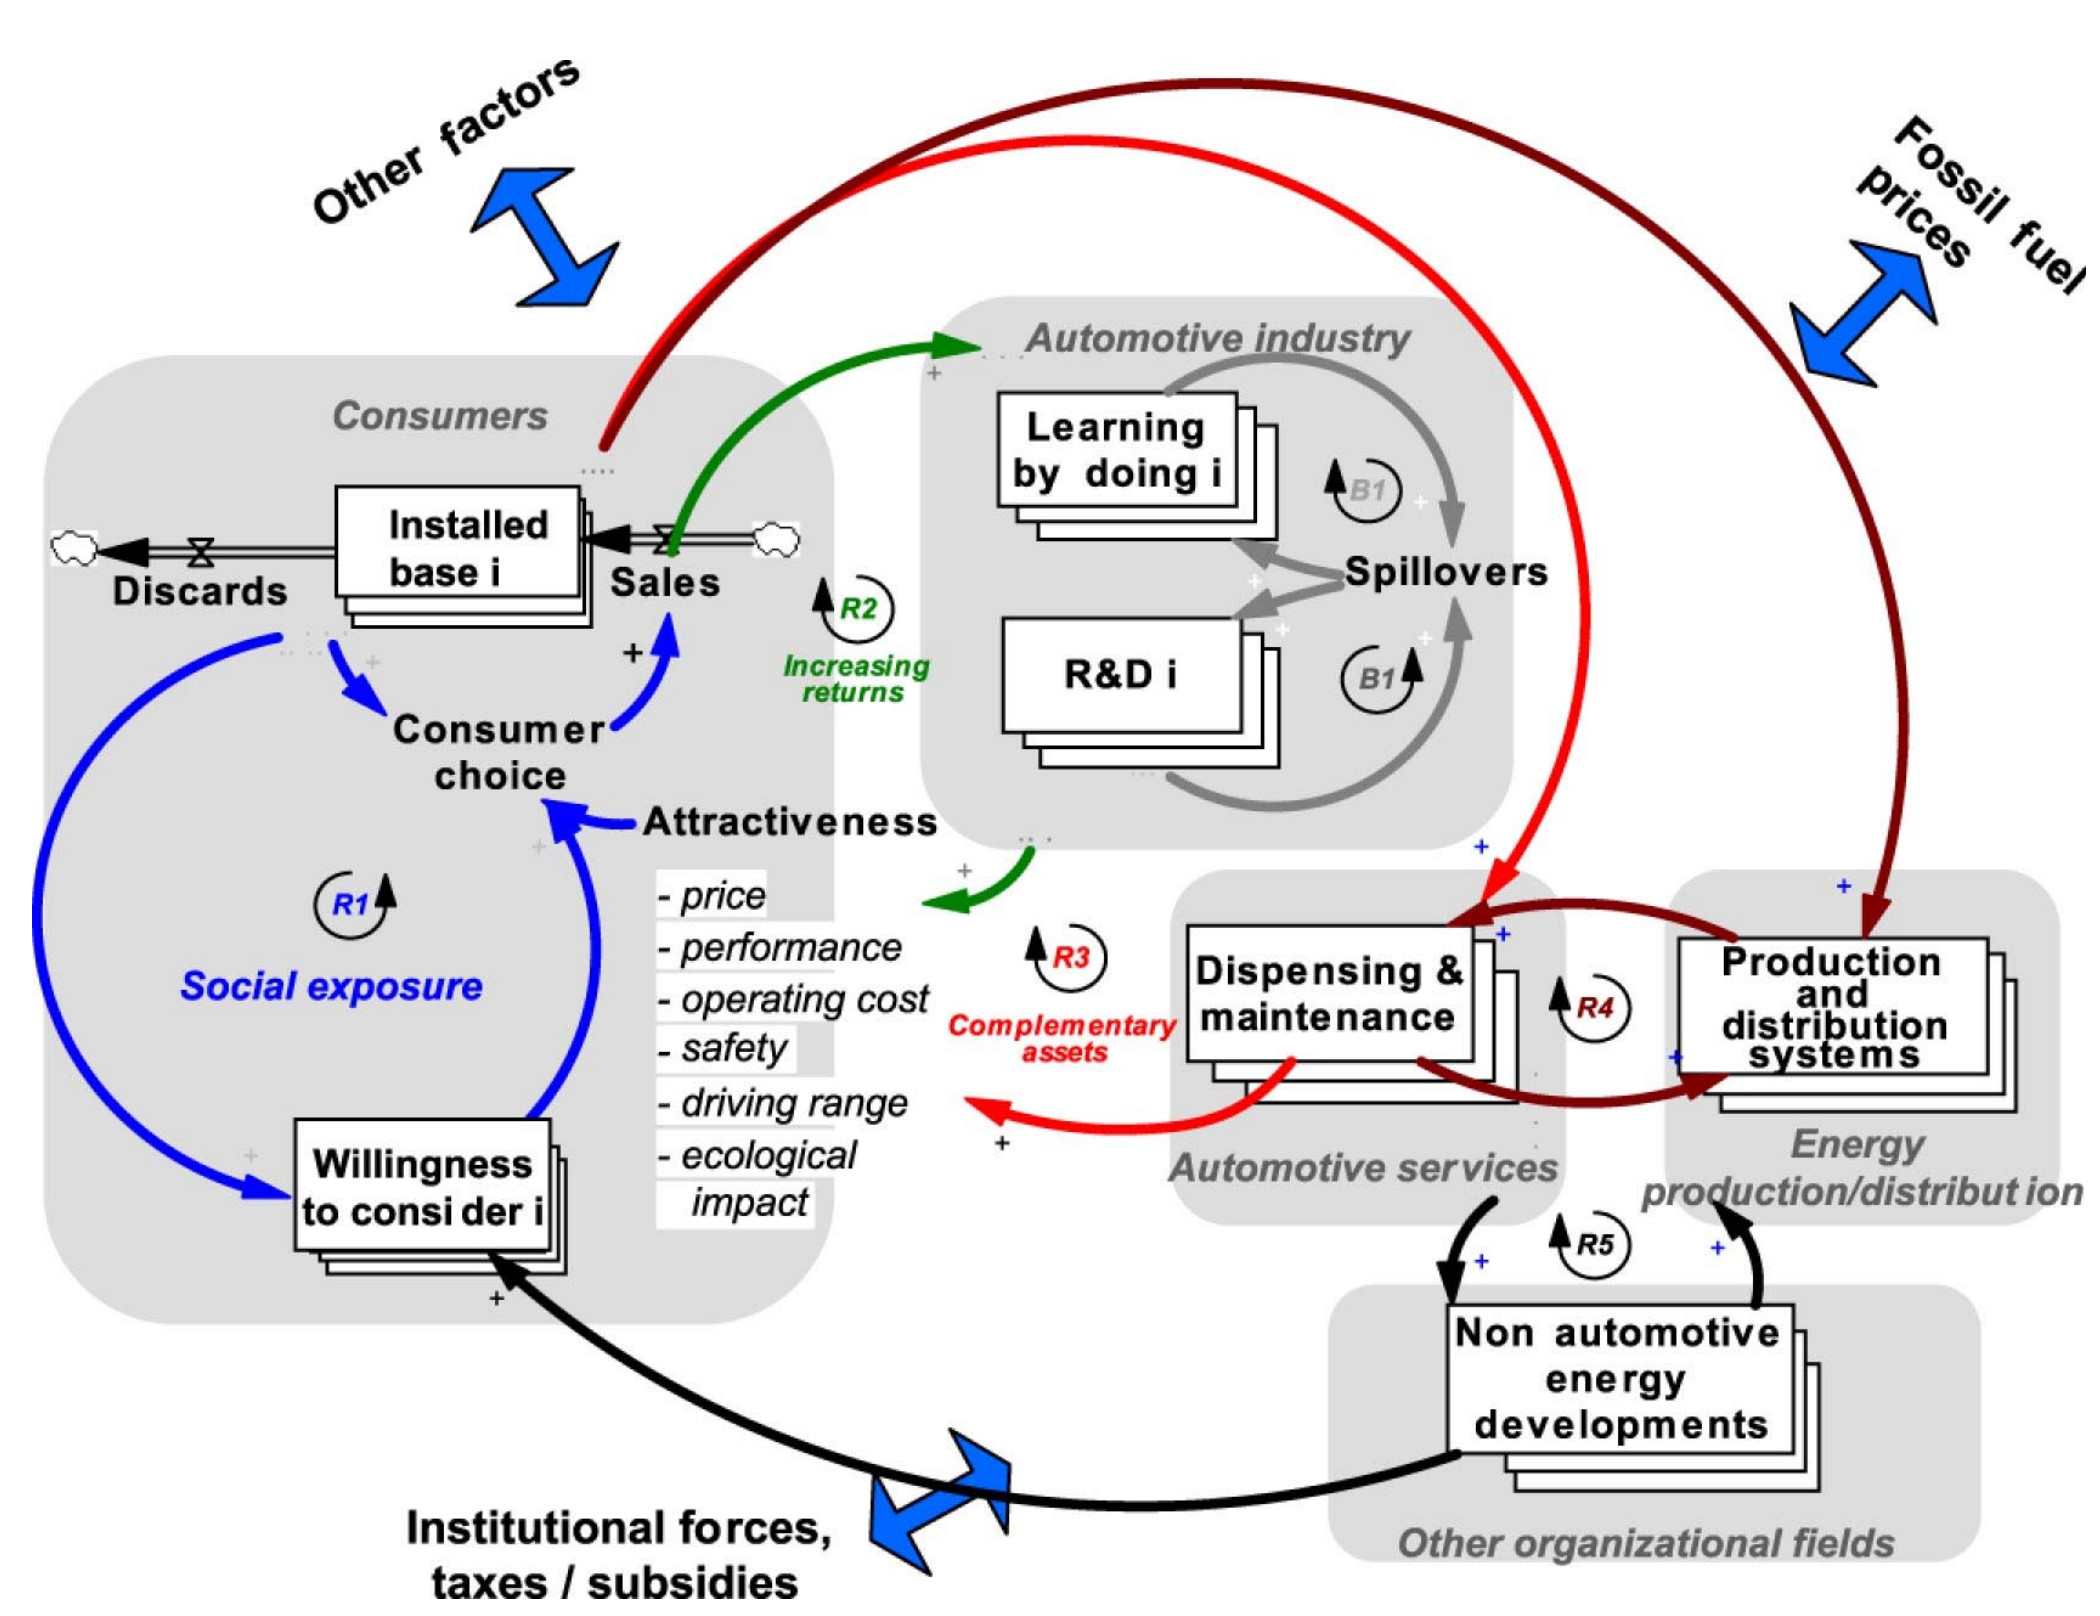
\includegraphics[height=\textheight]{Sterman-fig-2.jpg}
\end{frame}
    
\begin{frame}
  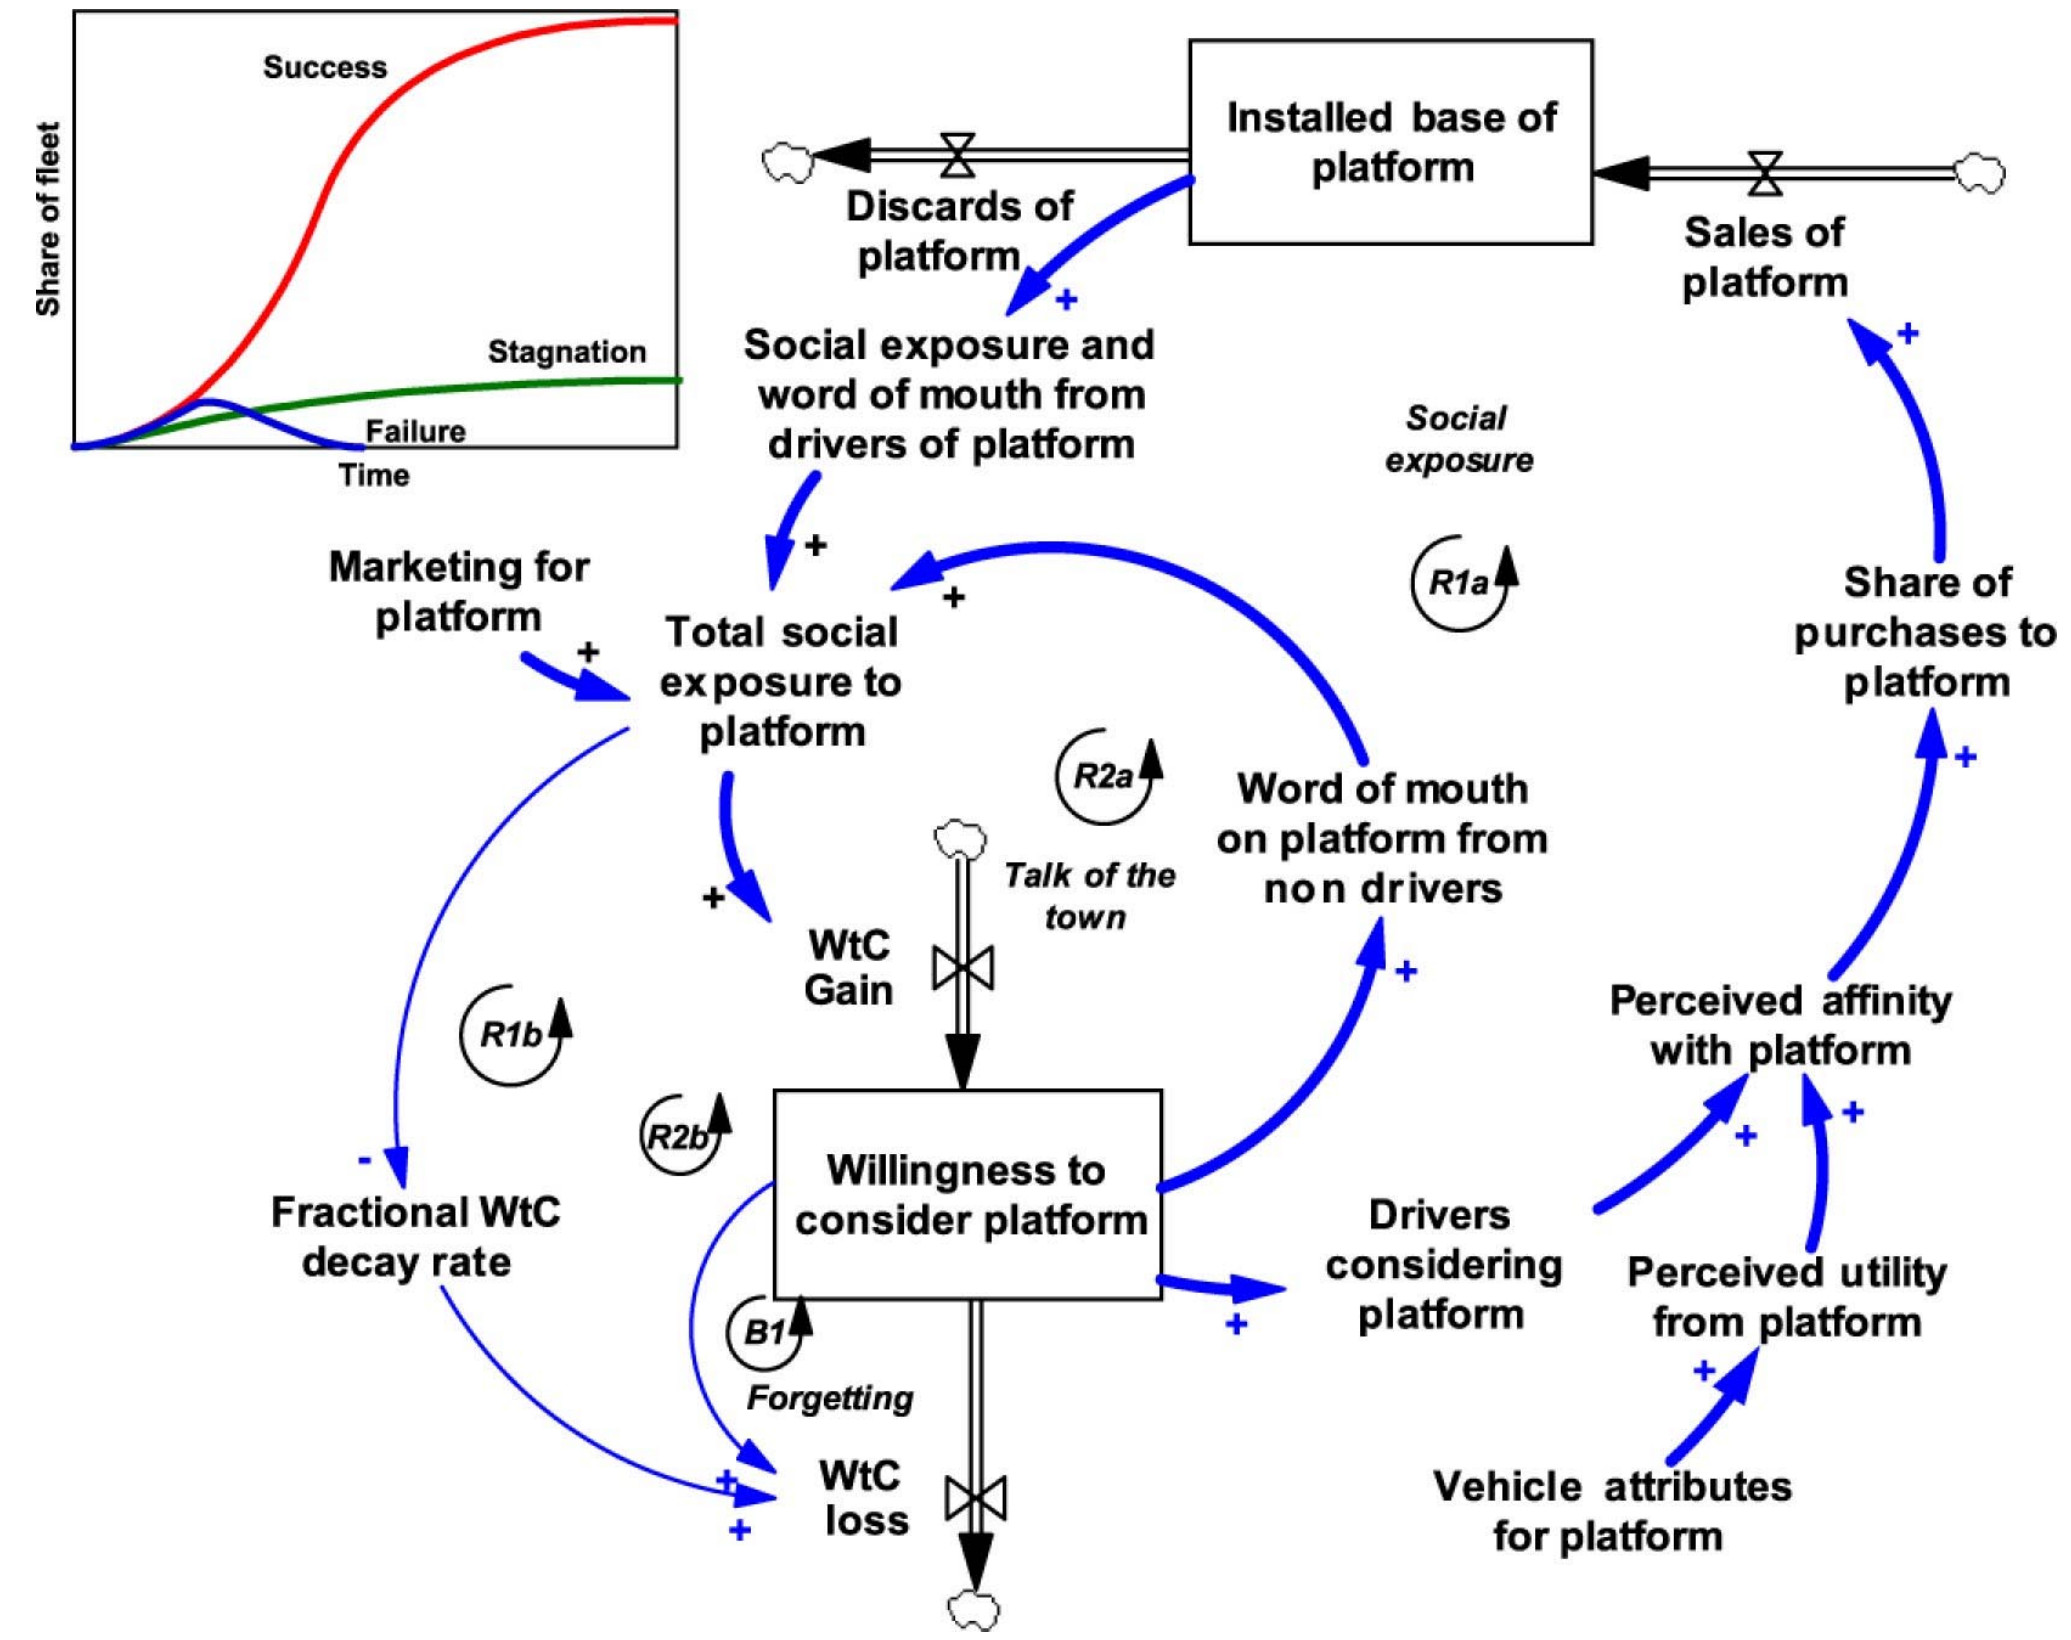
\includegraphics[height=\textheight]{Sterman-fig-3.jpg}
\end{frame}

\subsection{Results}

\begin{frame}
  \begin{eqnarray*}
    \frac{\mathrm{d}W_{ij}}{\mathrm{d}t}&=&\eta_{ij}(1-W_{ij})-\phi_{ij}W_{ij}\\
    \eta_{ij}&:& \textrm{Social exposure}\\
    \phi_{ij}&:& \textrm{Willingness-to-convert forgetfulness}
  \end{eqnarray*}

  \begin{center}
    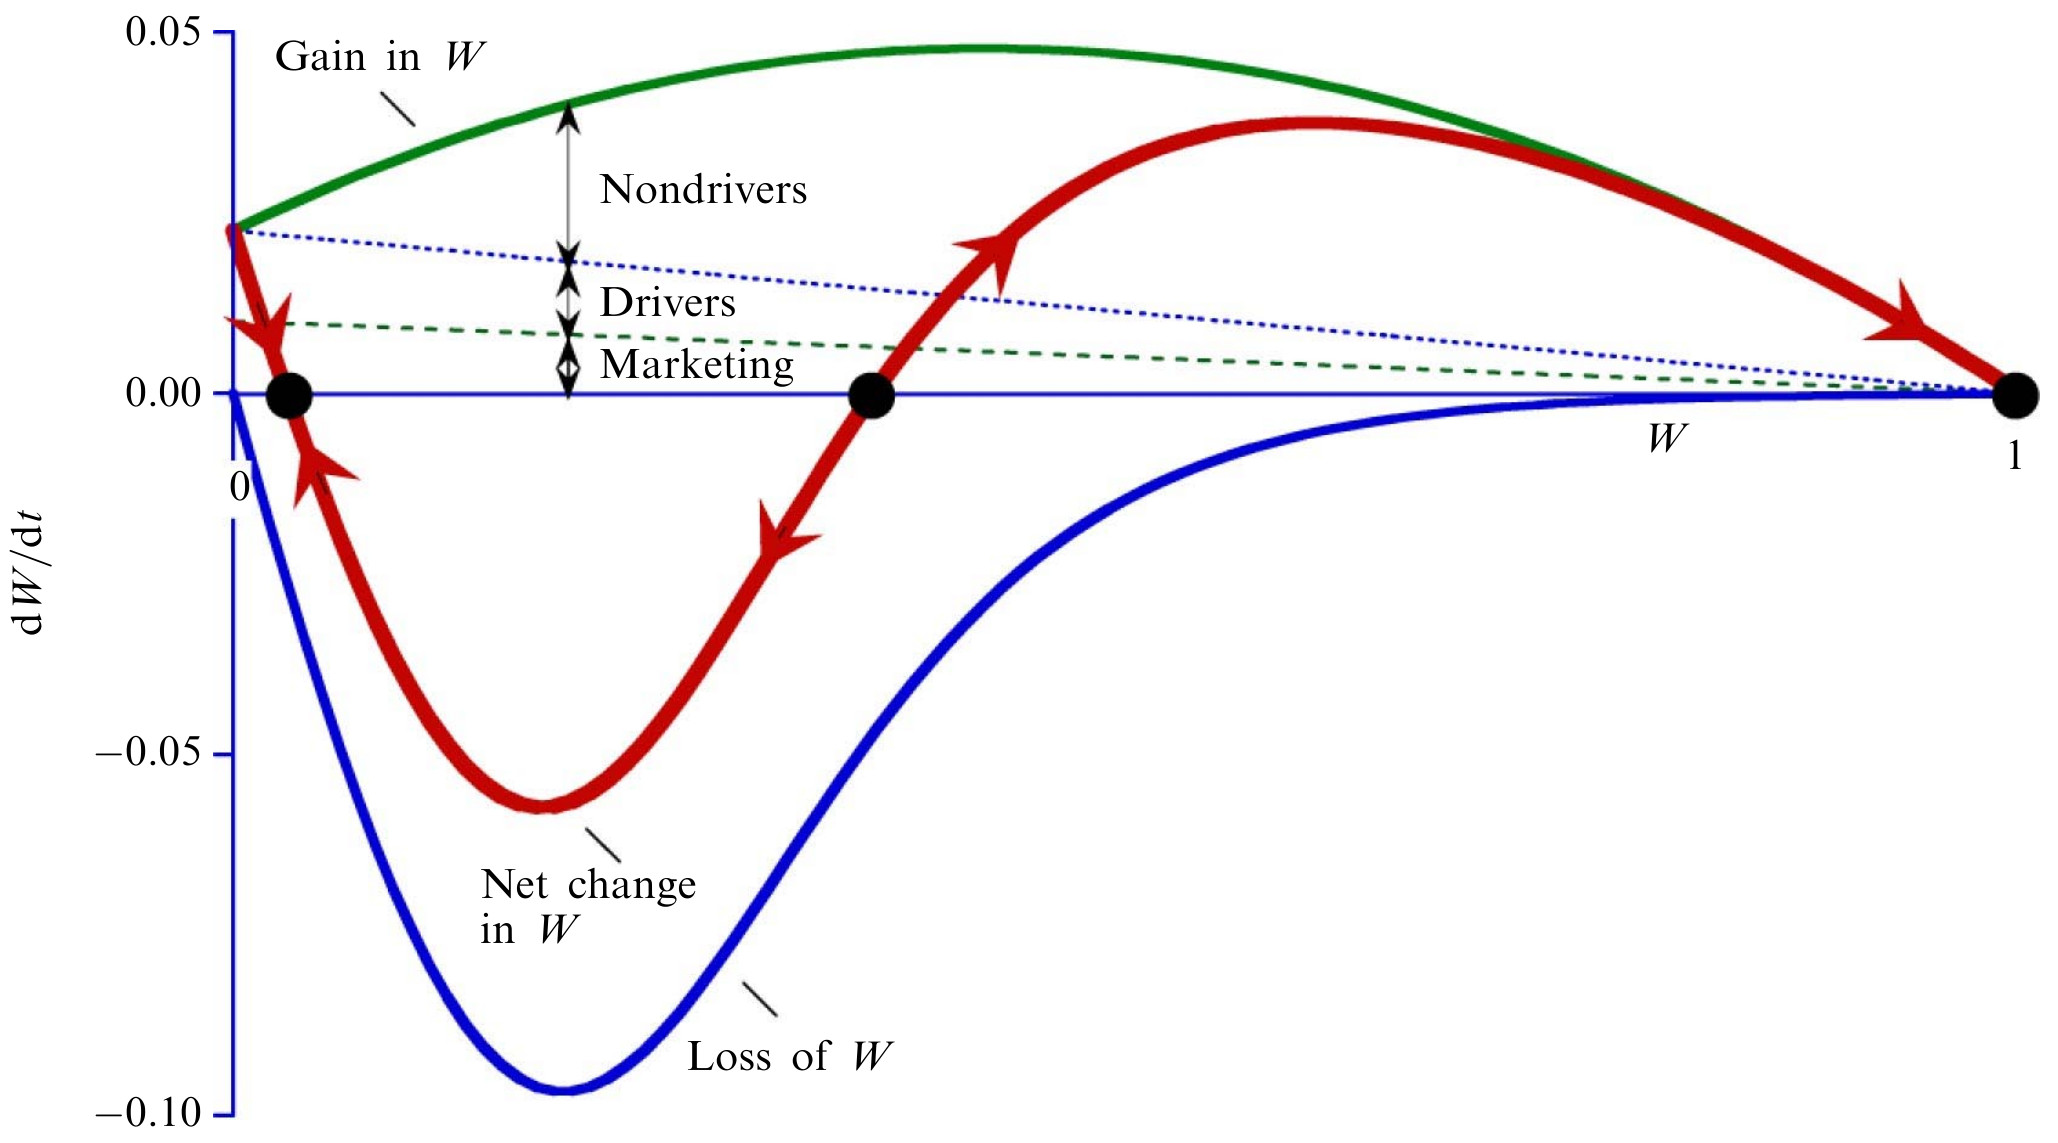
\includegraphics[width=0.8\textwidth]{Sterman-fig-4.jpg}
  \end{center}
\end{frame}
    
\begin{frame}
  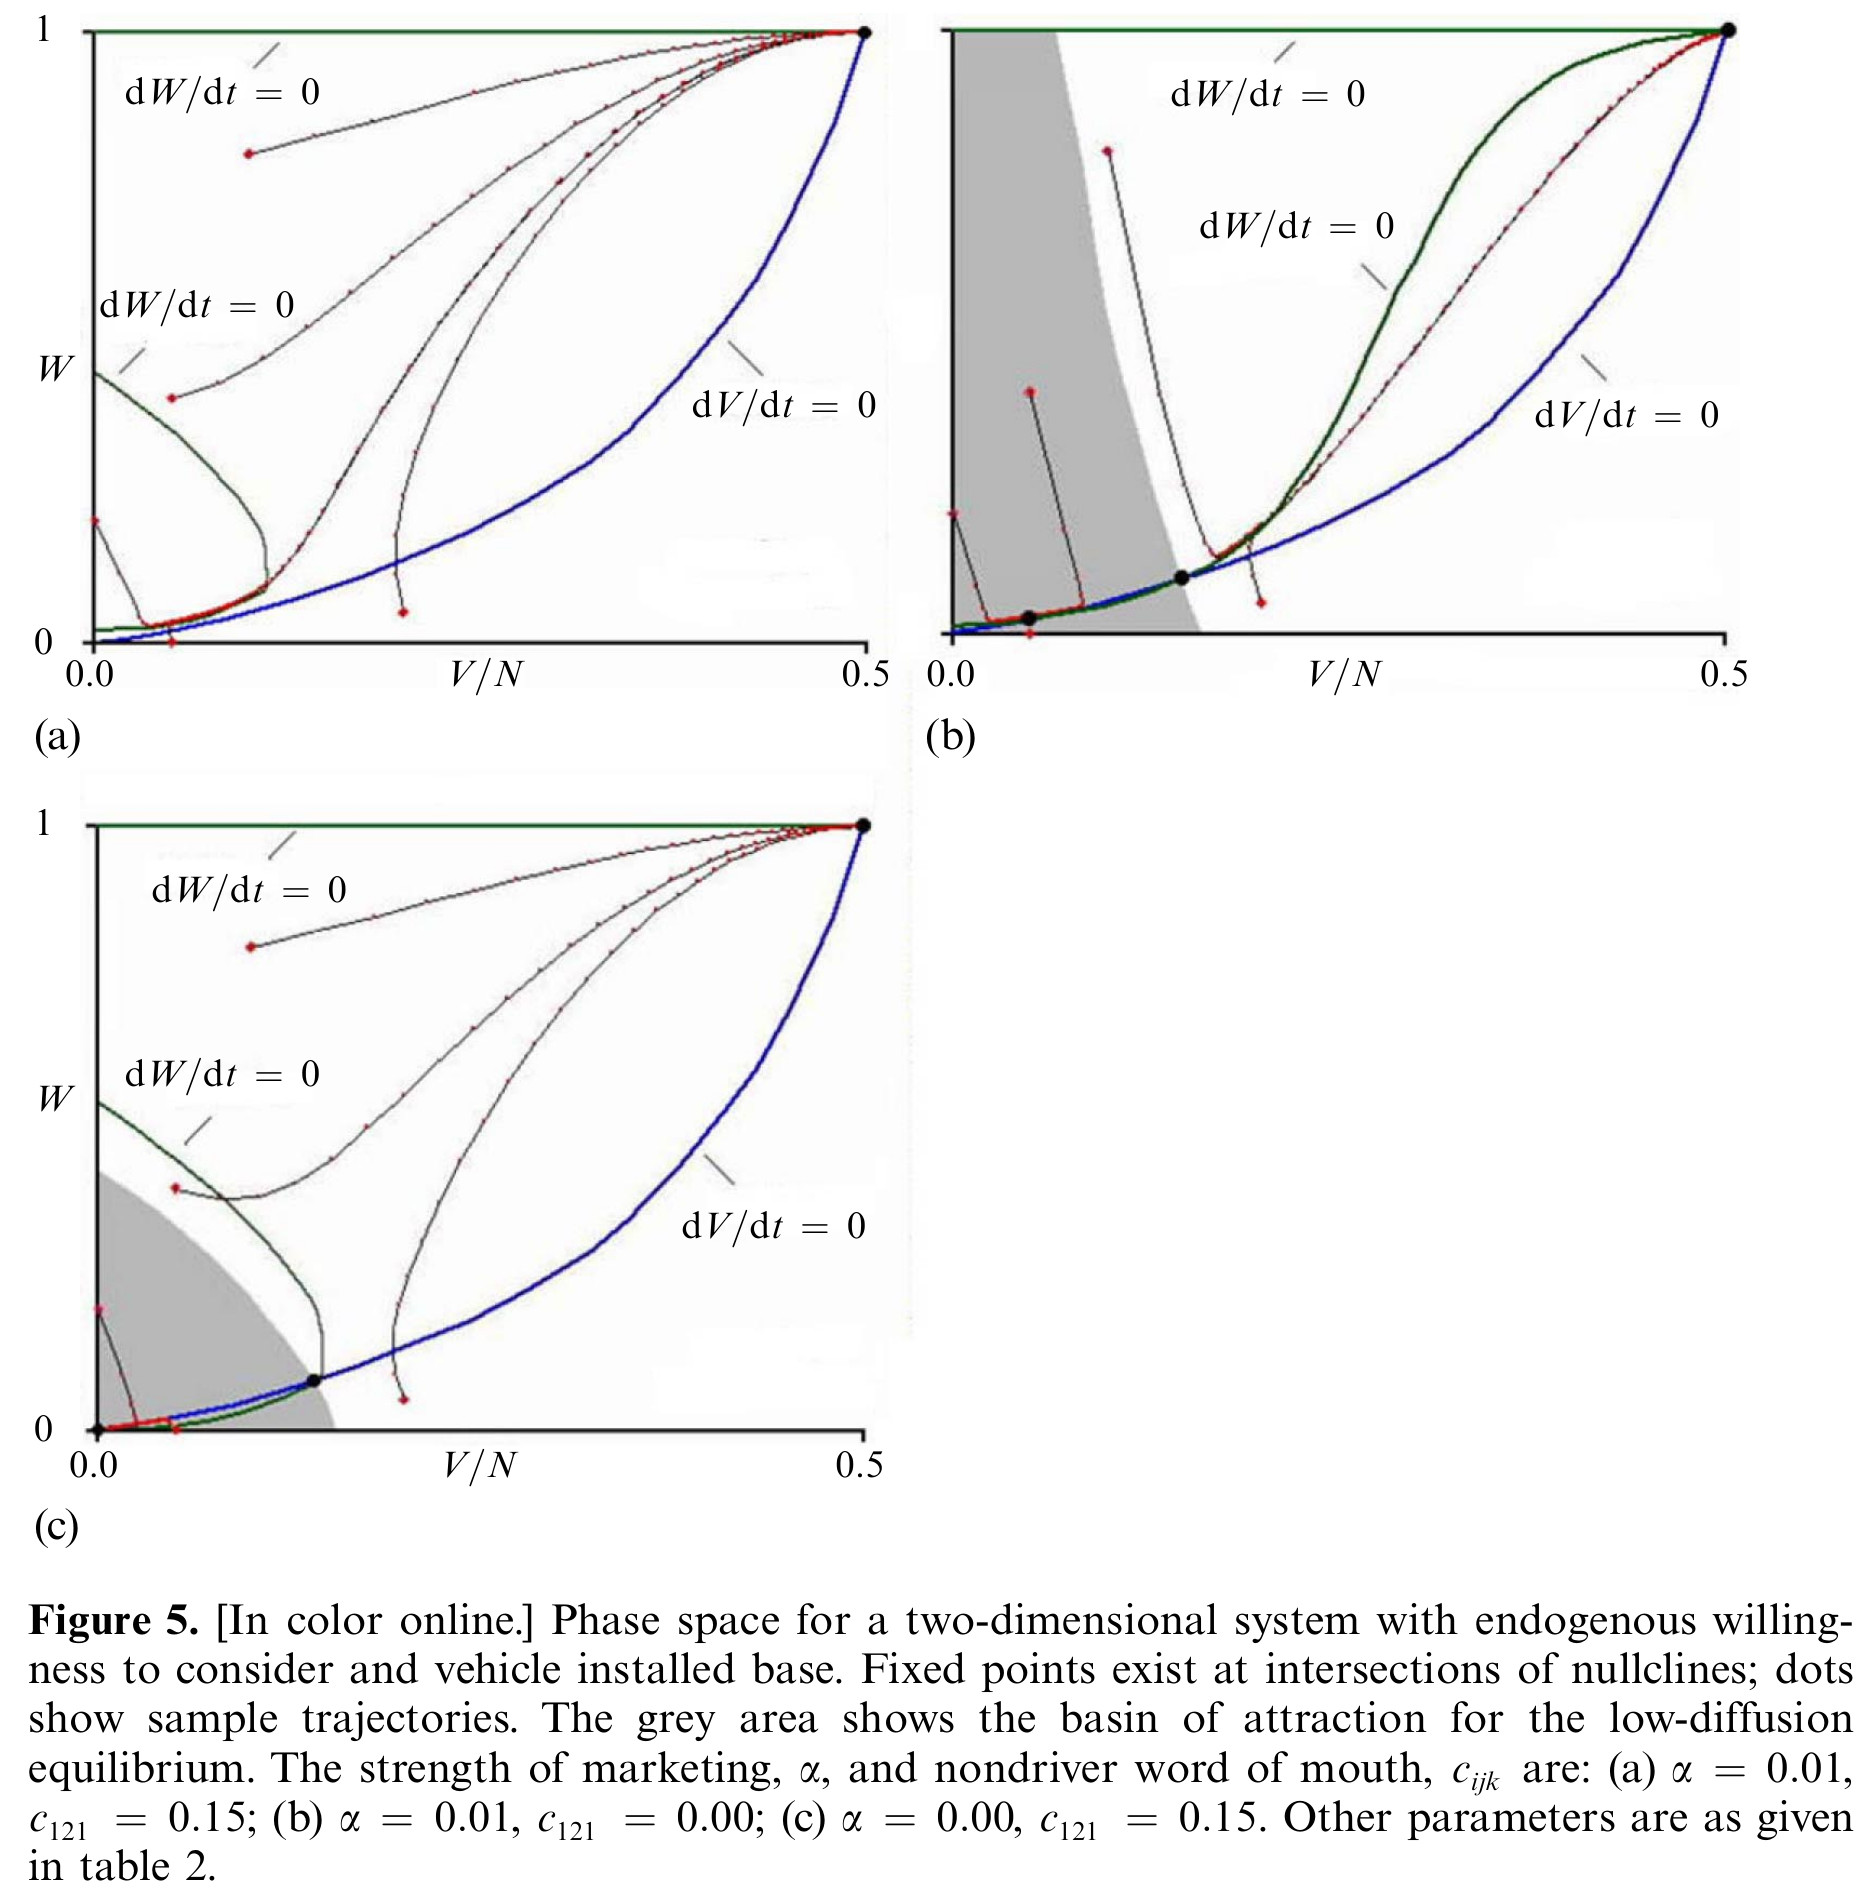
\includegraphics[height=\textheight]{Sterman-fig-5.jpg}
\end{frame}

\begin{frame}
  \begin{columns}
    \column{0.4\textwidth}
    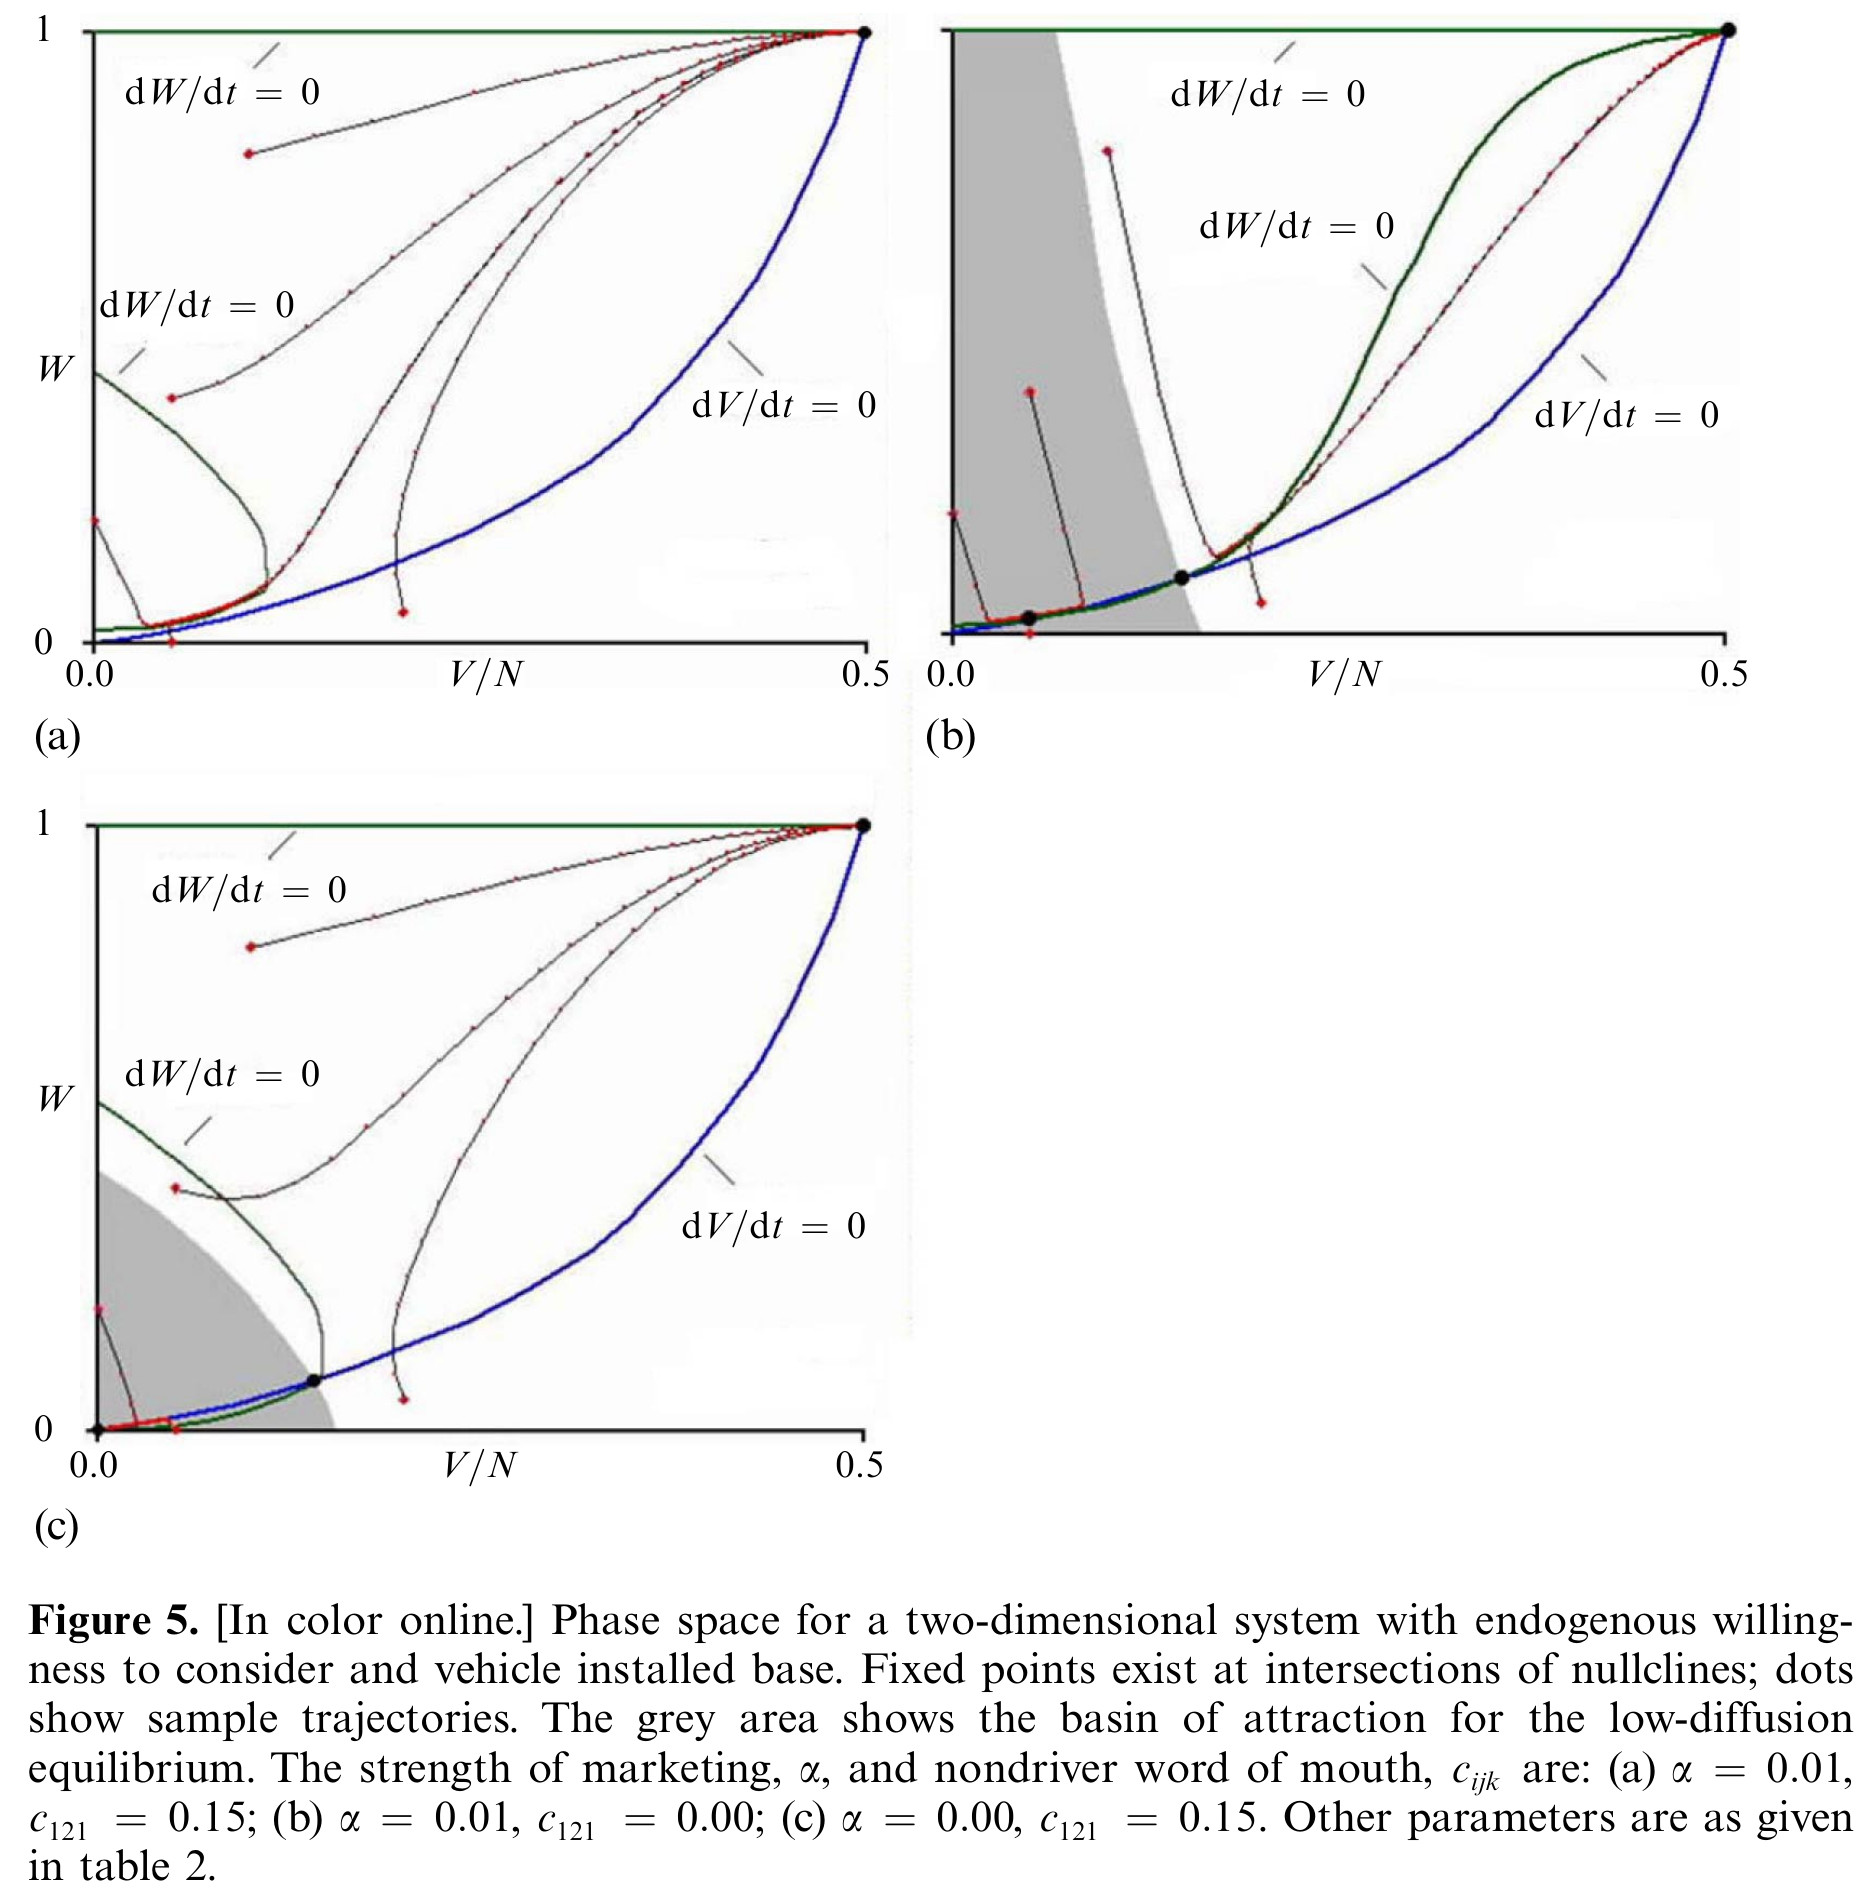
\includegraphics[width=\textwidth]{Sterman-fig-5.jpg}
    \column{0.6\textwidth}
    \begin{eqnarray*}
      \frac{\mathrm{d}V_{2}}{\mathrm{d}t}&=&\frac{\sigma_{22}V_2+\sigma_{12}(N-V_2)-V_2}{\lambda}\\
      \sigma_{i2}&=& \frac{W_{i2}a_{i2}}{W_{i1}a_{i1}+W_{i2}a_{i2}}\\
      a_{ij}&:&\textrm{affinity}
    \end{eqnarray*}
  \end{columns}
\end{frame}
    

\begin{frame}
  \includegraphics<+>[width=\textwidth]{Sterman-fig-6a.jpg}
  \includegraphics<+>[width=\textwidth]{Sterman-fig-6b.jpg}
  \includegraphics<+>[width=\textwidth]{Sterman-fig-6c.jpg}
\end{frame}


\begin{frame}
  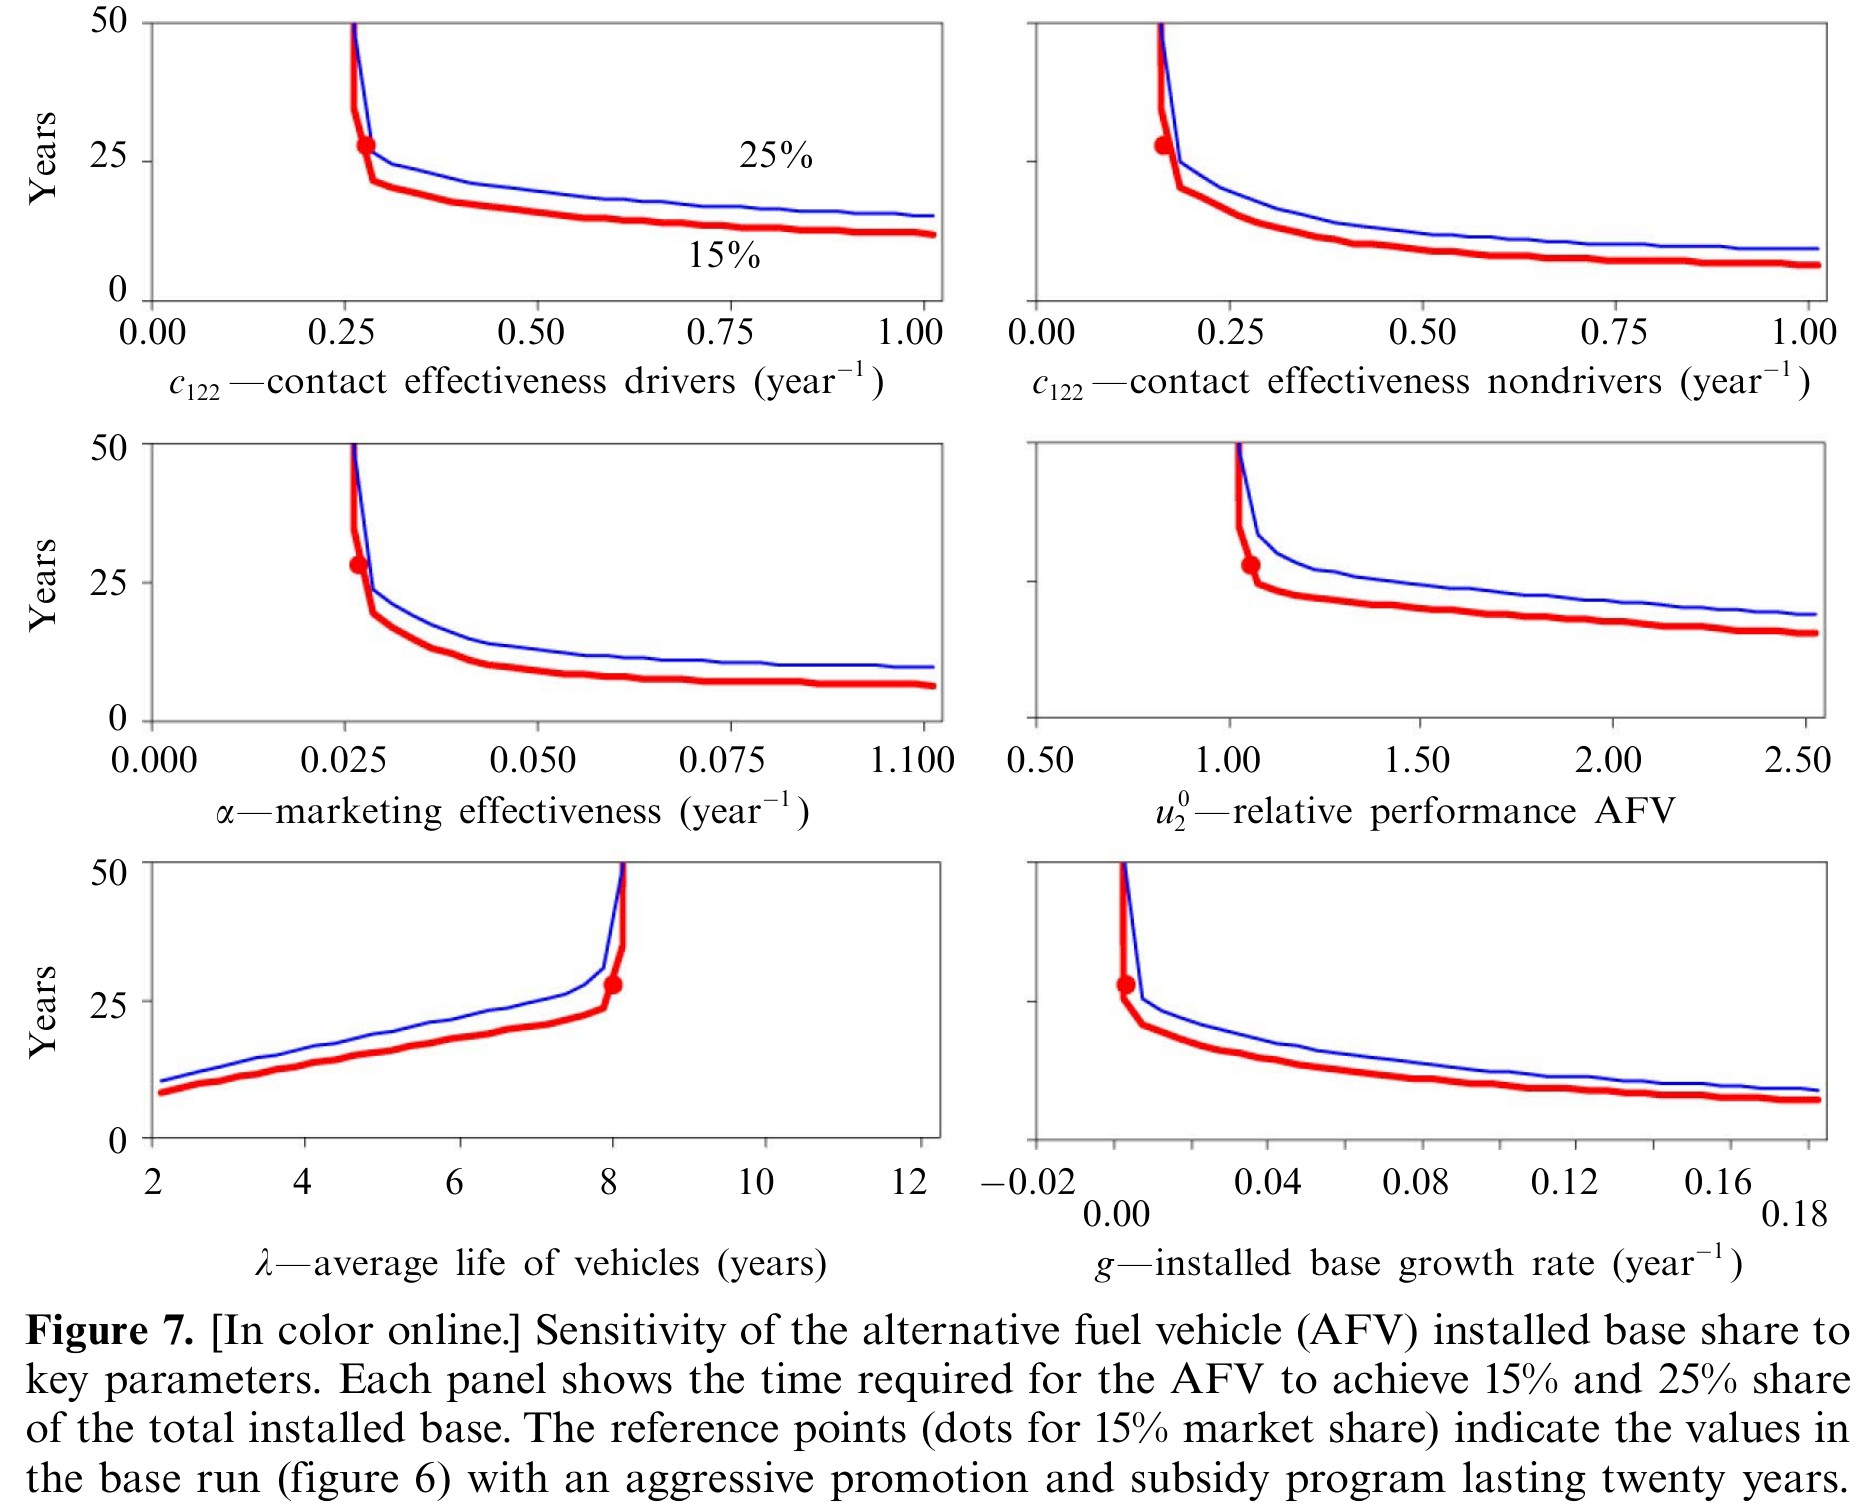
\includegraphics[height=\textheight]{Sterman-fig-7.jpg}
\end{frame}

\begin{frame}
  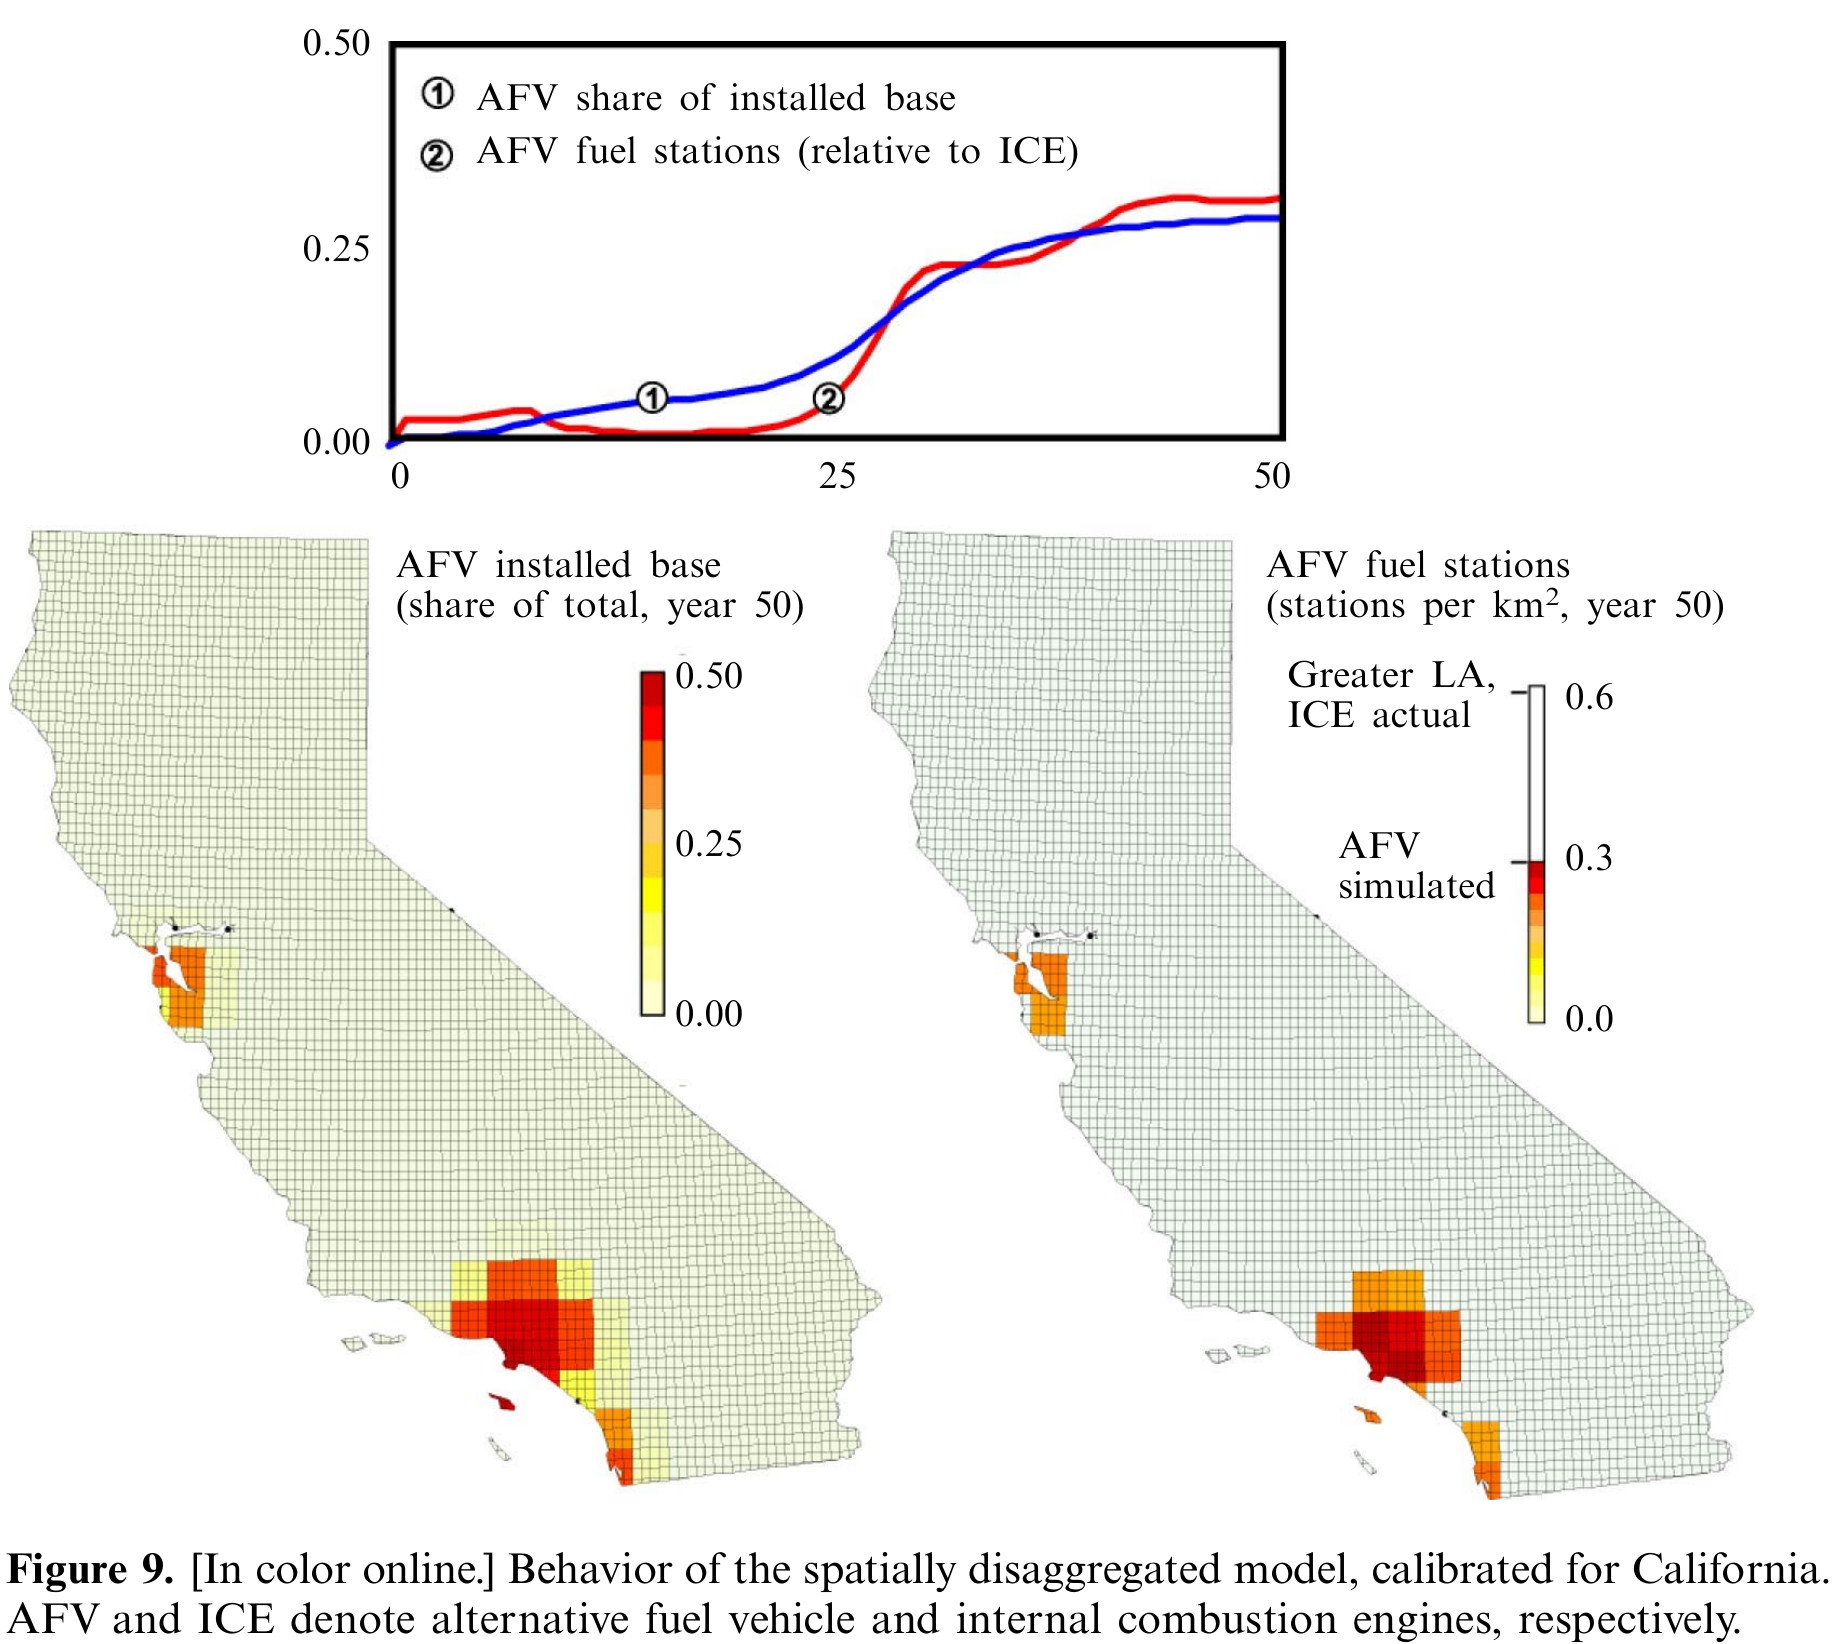
\includegraphics[height=\textheight]{Sterman-fig-9.jpg}
\end{frame}

\subsection{Discussion}
\begin{frame}
  \frametitle{Discussion}
  \begin{itemize}
  \item Installed base vs.~replacement rate vs.~cars-per-driver
  \item Car sharing may increase versatility
  \item How compelling would new cars have to be? (here $\leq 2.5$)
  \item Who Killed The Electric Car: why didn't competitors jump in?
  \item Didn't anticipate targeted advertisement
  \item cf. Tesla
  \end{itemize}
\end{frame}


%%%%%%%%%%%%%%%%%%%%%%%%%%%%%%%%%%%%%%%%%%%%%%%%%%%%%%%%%%%%%%%%%%%%%%

\section{Final points}
\begin{frame}
  \frametitle{Synergies}
  \begin{itemize}
  \item How does Struben\&Sterman's analysis relate to bike vs.~car?
  \item Are cars now improving exponentially? Fleet obsolescence:
    \begin{itemize}
    \item Self-driving: how compelling new cars are vs.~old (safety/insurance, opportunity cost\dots)?
    \item OTA updates: hardware ages, software is always new?
    \end{itemize}
  \end{itemize}
\end{frame}
  
  

\end{document}
